\documentclass{AeroStructure-ERJohnson}
\input crosslink.tex

\allowdisplaybreaks

%\usepackage{showframe}
\def\ShowFrameLinethickness{0.125pt}

\def\harp#1{\smash{\mathord{\buildrel{\lower3pt\hbox{$\scriptscriptstyle\rightharpoonup$}}\over{#1}}}}

\myexternaldocument{App_4P}
\myexternaldocument{Ch01_4P}
\myexternaldocument{Ch02_4P}
\myexternaldocument{Ch03_4P}
%\myexternaldocument{Ch04_4P}
\myexternaldocument{Ch05_4P}
\myexternaldocument{Ch06_4P}
\myexternaldocument{Ch07_4P}
\myexternaldocument{Ch08_4P}
\myexternaldocument{Ch09_4P}
\myexternaldocument{Ch10_4P}
\myexternaldocument{Ch11_4P}
\myexternaldocument{Ch12_4P}
\myexternaldocument{Ch13_4P}
\myexternaldocument{Ch14_4P}
\myexternaldocument{Ch15_4P}
\myexternaldocument{Ch16_4P}
\myexternaldocument{Ch17_4P}
\myexternaldocument{Ch18_4P}


\begin{document}


\mainmatter

%\hbox{~}\clearpage
%\setcounter{page}{1}

\setcounter{page}{71}
\setcounter{chapter}{3}

\chapter[Some aspects of the structural analysis]{Some aspects of the\break structural analysis} \label{ch4}

The thin-wall bar theory presented in chapter \ref{ch3} accounts for the deformations due to extension, bending, transverse shear, and torsion/twist. The inclusion of transverse shear strains is usually referred to as a Timoshenko bar theory. A summary of some of the equations from the theory is presented in article \ref{sec4.1}.

The von Mises criterion for yielding of a ductile metal under a combined stress state is reviewed in article \ref{sec4.2}. The permissible limits of the loads that prevent permanent deformation of the bar are determined by implementing the yield criterion.

In article \ref{sec4.3} we present examples to determine the axial displacement, axial normal strain, and axial normal stress, which include the following topics:
\begin{itemize}
 \item shear force and bending moment diagrams for distributed loads acting on a wing and a ship,
  \item the composite area technique to compute properties of plane areas,
  \item for a bar with a zee cross section, we determine the neutral axis of the cross section for the section subject to bending, the normal stress distribution, and the displacements due to pure bending and transverse bending.
\end{itemize}

In article \ref{sec4.4} the shear stresses are determined for several examples, including:
\begin{itemize}
  \item an open cross-sectional contour and a closed cross-sectional contour subject to a transverse shear force and a torque,
  \item comparison of an open section and equivalent closed section subject to torsion,
  \item resultant of a uniform shear flow and Bredt's formula,
  \item torsion of cross sections composed of two and three cells, and
  \item transverse bending of a bar with a two-cell cross section.
\end{itemize}

\newpage

\section{Review of the thin-wall bar theory}\label{sec4.1}

A straight bar is referenced to the Cartesian coordinate system \textit{x-y-z}, with the $z$-axis coinciding with the longitudinal axis of the bar. In the \textit{x-y} plane the cross section is described by the contour and the thickness of the wall normal to the contour. The contour is a piece-wise continuous curve in the \textit{x-y} plane whose subdivisions are called branches, and the tangent to the contour is continuous within a branch. The origin of the \textit{x-y} system in the cross section is at the centroid, which is the point labeled C in figure~\ref{fig4.1}. In the bar theory the dependent variables acting at the centroid the cross section of the bar are $[w(z), N(z)]$, $\left[\phi_{x}(z), M_{x}(z)\right]$, and $\left[\phi_{y}(z), M_{y}(z)\right]$. The axial displacement of the centroid is denoted by $w$ and its corresponding axial force is denoted by \textit{N}, the rotation of the cross section about the $x$-axis is denoted by $\phi_{x}$ and its corresponding bending moment is denoted by $M_{x}$, and the rotation about the negative $y$-axis is denoted by $\phi_{y}$ and its corresponding bending moment is denoted by $M_{y}$. The shear center of the cross section is labeled S.C. in figure~\ref{fig4.1}, and the dependent variables acting at the shear center are $\left[u(z), V_{x}(z)\right]$, $\left[v(z), V_{y}(z)\right]$, and $\left[\phi_{z}(z), M_{z}(z)\right]$. The $x$-direction displacement of the shear center is denoted by $u$ and its corresponding force by $V_{x}$, the $y$-direction displacement of the shear center is denoted by $v$ and its corresponding force by $V_{y}$, and the twist of the cross section is denoted by $\phi z$ and its associated\break torque~by~$M_{z}$.

{\def\thefigure{4.1}
\processfigure[H]{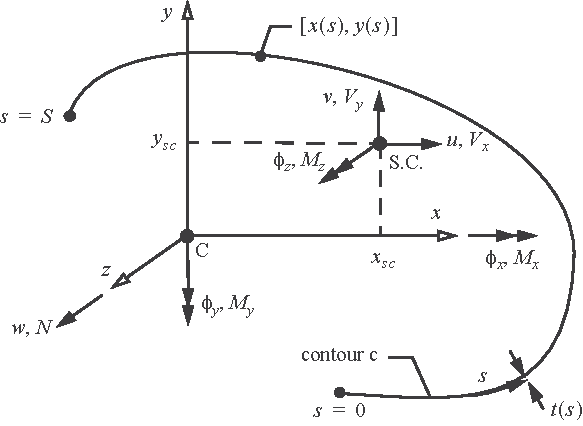
\includegraphics{Figure_4-1.pdf}
}{\caption{Coordinate
systems in the bar theory, and the dependent\break variables referenced to the~cen\-troid~and the shear center of the cross section.\label{fig4.1}}}}


\subsection{Extension and bending}\label{sec4.1.1}

Hooke's law for extension and bending of the bar is defined relative
to the centroid. From eq.~(\ref{eq3.80}) on page~\pageref{eq3.80} the compliance form of Hooke's law is
\begin{align}\label{eq4.1}
\left[\begin{array}{@{}l@{}}d w/d z \\d \phi_{x}/d z \\d \phi_{y}/d z\end{array}\right]=\frac{1}{E}\left[\begin{array}{@{}ccc@{}}1/A & 0 & 0 \\0 & k/I_{x x} & \left(-k n_{x}\right)/I_{y y} \\0 & \left(-k n_{y}\right)/I_{x x} & k/I_{y y}\end{array}\right]\left[\begin{array}{@{}c@{}}N+N_{T} \\M_{x}+M_{x T} \\M_{y}+M_{y T}\end{array}\right].
\end{align}
Geometric properties of the cross section are its area \textit{A}, its first area moments $Q_{x}$ and $Q_{y}$, and its second area moments $I_{xx}, I_{yy}$, and $I_{xy}$. In eq.~(\ref{eq4.1}) the modulus of elasticity of the material is denoted by \textit{E}. The locus of points on the contour is expressed parametrically by the equations $x(s)$ and $y(s)$, where the arc-length of the contrary is denoted by $s$. Let $t(s)$ denote the thickness of the contour. See Fig.~\ref{fig4.1}. The area and first area moments are given~\vspace*{4pt}by\pagebreak
\begin{align}\label{eq4.2}
A=\int_{c} t(s) d s \quad Q_{x}=\int_{c} y(s) t(s) d s=0 \quad Q_{y}=\int_{c} x(s) t(s) d s=0.
\end{align}
First area moments $Q_{x}$ and $Q_{y}$ vanish since origin of the \textit{x-y}-axes is located at the centroid of the cross section. Hence, the definition of the centroid allows decoupling of the extension and bending responses of the bar. That is, the axial strain $d w/d z$ is independent of the bending moments $M_{x}$ and $M_{y}$, and bending rotation gradients $d \phi_{x}/d z$, and $d \phi_{y}/d z$ are independent of axial force $N$. The second area moments are given by,
\begin{align}\label{eq4.3}
I_{x x}=\int_{c} y^{2}(s) t(s) d s \quad I_{y y}=\int_{c} x^{2}(s) t(s) d s \quad I_{x y}=\int_{c} x(s) y(s) t(s) ds.
\end{align}
The dimensionless parameters are defined by
\begin{align}\label{eq4.4}
n_{x}=I_{x y}/I_{x x} \quad n_{y}=I_{x y}/I_{y y} \quad k=\frac{1}{1-n_{x} n_{y}}.
\end{align}
The thermal loads $N_{T}$, $M_{x T}$, and $M_{y T}$ appearing in eq.~(\ref{eq4.1}) are from the prescribed change in temperature from the reference state. Refer to eqs. (\ref{eq3.75}), and (\ref{eq3.78}) on page \pageref{eq3.75}.


The axial normal stress $\sigma_{z z}$ and the shear stress tangent to the contour $\sigma_{z s}$ are shown in figure~\ref{fig4.2}. The axial normal strain $\varepsilon_{z z}$ and the axial normal stress $\sigma_{z z}$ are given by eqs. (\ref{eq3.82}) and (\ref{eq3.83}) on page \pageref{eq3.82}, respectively. These results are repeated below as eqs. (\ref{eq4.5}) and (\ref{eq4.6}), respectively.
{\def\thefigure{4.2}
\processfigure[H]{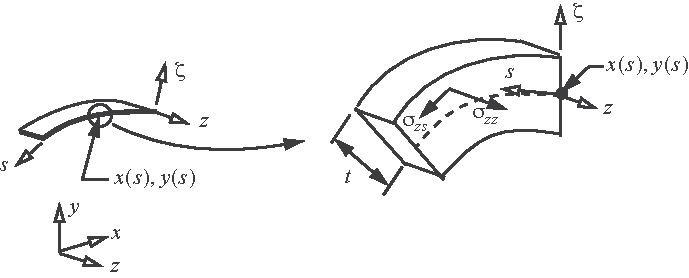
\includegraphics{Figure_4-2.pdf}
}{\caption{Dominant stresses acting on the z-face in a thin-walled bar.\label{fig4.2}}}}
\vspace*{-2\baselineskip}
\begin{align}\label{eq4.5}
\varepsilon_{z z}=\frac{N+N_{T}}{E A}+k \frac{\left(M_{x}+M_{x T}\right)}{E I_{x x}} \bar{y}(s)+k \frac{\left(M_{y}+M_{y T}\right)}{E I_{y y}} \bar{x}(s),\ \text{and}\\
\label{eq4.6}
\sigma_{z z}=\frac{N+N_{T}}{A}+k \frac{\left(M_{x}+M_{x T}\right)}{I_{x x}} \bar{y}(s)+k \frac{\left(M_{y}+M_{y T}\right)}{I_{y y}} \bar{x}(s)-\beta \Delta T(s, z).
\end{align}
In eq.~(\ref{eq4.6}) $\beta=E \alpha$, where $\alpha$ is the linear coefficient of thermal expansion of the material. The cross-sectional coordinates of the contour $\bar{x}(s)$ and $\bar{y}(s)$ appearing in eq.~(\ref{eq4.6}) are defined by
\begin{align}\label{eq4.7}
\bar{x}(s)=x(s)-n_{x} y(s) \quad \bar{y}(s)=y(s)-n_{y} x(s).
\end{align}

\subsection{Shear stresses in open and closed sections}\label{sec4.1.2}

The location of the shear center and the equation for the shear stress depend on whether the cross-sectional contour is open or closed.

\subsubsection*{Open cross-sectional contour} The coordinates of the shear center with respect to the centroid for an open cross-sectional contour are given by
\begin{align}\label{eq4.8}
x_{s c}=-\left(\frac{k}{I_{x x}}\right)\left[\int_{c} r_{n c}(s) \bar{Q}_{x}(s) d s\right] \quad y_{s c}=\frac{k}{I_{y y}}\left[\int_{c} r_{n c}(s) \bar{Q}_{y(s)} d s\right].
\end{align}
In eq.~(\ref{eq4.8}) the functions denoted by $\bar{Q}_{x}(s)$ and $\bar{Q}_{y}(s)$ are called distribution functions. The equations for the distribution functions are
\begin{align}\label{eq4.9}
\bar{Q}_{x}(s)=\int_{0}^{s}[\bar{y}(s) t(s)] d s \quad \bar{Q}_{y}(s)=\int_{0}^{s}[\bar{x}(s) t(s)] d s.
\end{align}
In eq.~(\ref{eq4.8}) the coordinate normal to the contour with respect to the centroid is denoted by $r_{n c}(s)$. Coordinate $r_{n c}(s)$ is shown in figure~\ref{fig3.3}(b) on page \pageref{fig3.3}, which is given by
\begin{align}\label{eq4.10}
r_{n c}(s)=x(s) \frac{d y}{d s}-y(s) \frac{d x}{d s}.
\end{align}
Also shown in figure~\ref{fig3.3}(b) is the coordinate normal to the contour with respect to the shear center which is denoted by $r_{n}(s)$. It is given by
\begin{align}\label{eq4.11}
r_{n}(s)=r_{n c}(s)-x_{s c} \frac{d y}{d s}+y_{s c} \frac{d x}{d s}.
\end{align}
The shear stress $\sigma_{z s}$ for an open cross-sectional contour consists of the sum of two terms, and it is given by
\begin{align}\label{eq4.12}
\sigma_{z s}=\frac{q(s, z)}{t(s)}+2 \frac{M_{z}(z)}{J} \zeta \quad-t/2 \leq \zeta \leq t/2.
\end{align}
where the shear flow is denoted by $q(s, z)$, the torsion constant by \textit{J}, and the thickness coordinate by $\zeta$. The shear flow for an open section is related to the distribution functions and the shear forces by
\begin{align}\label{eq4.13}
q(s, z)=-\frac{k}{I_{y y}} \bar{Q}(s) V_{x}(z)-\frac{k}{I_{x x}} \bar{Q}_{x}(s) V_{y}(z).
\end{align}
The first term on the right-hand side of eq.~(\ref{eq4.12}) is the shear stress component that varies with the contour coordinate $s$, but it is independent of the thickness coordinate $\zeta$. The second term on the right-hand side of eq.~(\ref{eq4.12}) is a linear function of the thickness coordinate $\zeta$, but it is independent of the contour coordinate $s$ in a branch of the cross section where the torsion constant is spatially uniform. The torsion constant is derived in article \ref{sec3.9} on page \pageref{sec3.9} and in article \ref{sec3.9.1}. For thin-wall bars it is given by
\begin{align}\label{eq4.14}
J=\sum_{\textrm{branches }} \frac{1}{3} b_{i} t_{i}^{3},
\end{align}
where $b_{i}$ is the arc-length of the \textit{i-th} branch and $t_{i}$ is the thickness of the \textit{i-th} branch.

\subsubsection*{Closed cross-sectional contour.} We begin with the shear flow given by eq.~(\ref{eq3.145}) on page~\pageref{eq3.145}, which is repeated below as eq.~(\ref{eq4.15}).
\begin{align}\label{eq4.15}
q(s, z)=q_{0}(z)-\frac{k}{I_{y y}} V_{x} \bar{Q}_{y}(s)-\frac{k}{I_{x x}} V_{y} \bar{Q}_{x}(s).
\end{align}\vspace*{3pt}
\clearpage

\noindent The shear flow $q_{0}(z)$ is spatially uniform around the contour, and it is determined from
\begin{align}\label{eq4.16}
M_{z c}=\oint\kern-2pt r_{n c}(s) q(s) d s,
\end{align}
where the torque with respect to the centroid is denoted by $M_{z c}$. Substitute eq.~(\ref{eq4.15}) for the shear flow into eq.~(\ref{eq4.16}) and solve for $q_{0}(z)$. The shear flow with respect to the centroid is expressed as
\begin{align}\label{eq4.17}
q_{C}(s, z)=\frac{M_{z c}(z)}{2 A_{c}}-F_{x c}(s) V_{x}(z)-F_{y c}(s) V_{y}(z),
\end{align}
where $A_{c}$ is the area enclosed by the contour, and functions $F_{x c}(s)$ and $F_{y c}(s)$ account for the distribution of the shear flow due to the transverse shear forces. It is tacitly implied that the torque $M_{z c}$ and shear forces $V_{x}$ and $V_{y}$ are resolved at the centroid in the derivation of the shear flow given by eq.~(\ref{eq4.17}). Then the area enclosed by the contour is given by
\begin{align}\label{eq4.18}
A_{c}=\frac{1}{2} \oint\! r_{n c}(s) d s.
\end{align}
The shear flow distribution functions relative to the centroid appearing in eq.~(\ref{eq4.17}) are defined by
\begin{align}\label{eq4.19}
F_{x c}(s)=\frac{k}{I_{y y}}\left[\bar{Q}_{y}(s)-\frac{1}{\left(2 A_{c}\right)} \oint\! r_{n c}(s) \bar{Q}_{y}(s) d s\right] \quad F_{y c}(s)=\frac{k}{I_{x x}}\left[\bar{Q}_{x}(s)-\frac{1}{\left(2 A_{c}\right)} \oint\! r_{n c}(s) \bar{Q}_{x}(s) d s\right].
\end{align}
The twist per unit longitudinal length due to torsion for a closed cell is derived in article \ref{sec3.11.1} on page \pageref{sec3.11.1}. It is an important equation and is given by
\begin{align}\label{eq4.20}
\frac{d \phi_{z}}{d z}=\frac{1}{2 A_{c}} \oint\left(\frac{q}{G t}\right) d s,
\end{align}
where the shear modulus of the material is denoted by \textit{G}. From figure~\ref{fig3.23} on page~\pageref{fig3.23}, the torque at the shear center is related to the torque at the centroid and the shear forces acting at the shear center by
\begin{align}\label{eq4.21}
M_{z}=M_{z c}-x_{s c} V_{y}+y_{s c} V_{x}.
\end{align}
Substitute the shear flow from eq.~(\ref{eq4.17}), and substitute the torque at the centroid from eq.~(\ref{eq4.21}), into eq.~(\ref{eq4.20}) to find
\begin{align}\label{eq4.22}
\frac{d \phi_{z}}{d z}=\frac{M_{z}}{4 A_{c}^{2}} \oint\! \frac{d s}{G t}-\left[\frac{y_{s c}}{4 A_{c}^{2}} \oint\! \frac{d s}{G t}+\frac{1}{2 A_{c}} \oint\! \frac{F_{x c}}{G t} d s\right] V_{x}+\left[\frac{x_{s c}}{4 A_{c}^{2}} \oint\! \frac{d s}{G t}-\frac{1}{2 A_{c}} \oint\! \frac{F_{y c}}{G t} d s\right] V_{y}.
\end{align}
At the shear center the twist per unit length depends on the torque resolved at the shear center and not on the shear forces. In other words, the shear forces acting at the shear center do not contribute to torsion. This requirement means the coefficients of the shear forces in eq.~(\ref{eq4.22}) must vanish. Hence, the location of the shear center with respect to the centroid is
\begin{align}\label{eq4.23}
x_{s c}=\left[\frac{2 A_{c}}{\oint\! \frac{d s}{G t}} \oint\left(\frac{F_{y c}(s)}{G t}\right) d s\right] \quad y_{s c}=-\left[\frac{2 A_{c}}{\oint\! \frac{d s}{G t}} \oint\left(\frac{F_{x c}(s)}{G t}\right) d s\right].
\end{align}
It follows from eq.~(\ref{eq4.22}) that the twist per unit length is related to the torque by
\[\frac{d \phi_{z}}{d z}=\frac{M_{z}}{(G J)_{\mathrm{eff}}},\]
\vspace*{3pt}
\clearpage

\noindent where the effective torsional stiffness is given by
\begin{align}\label{eq4.24}
(G J)_{\mathrm{eff}}=\frac{4 A_{c}^{2}}{\oint\! \frac{d s}{G t}}.
\end{align}
The shear flow defined with respect to the shear center is obtained as follows: Substitute eq.~(\ref{eq4.21}) for the torque acting at the centroid into the shear flow eq.~(\ref{eq4.17}) to get the result
\begin{align}\label{eq4.25}
q(s, z)=\frac{M_{z}(z)}{2 A_{c}}-F_{x}(s) V_{x}(z)-F_{y}(s) V_{y}(z),
\end{align}
where the shear flow distribution functions relative to the shear center are defined by
\begin{align}\label{eq4.26}
F_{x}(s)=\frac{y_{s c}}{2 A_{c}}+F_{x c}(s) \quad F_{y}(s)=-\left(\frac{x_{s c}}{2 A_{c}}\right)+F_{y c}(s).
\end{align}
The shear stress for a closed cross-sectional contour is given by $\sigma_{z s}=q(s, z)/t(s)$. Note that the shear stress is uniform through the thickness of the wall but is a function of the contour coordinate.


\subsection{Hooke's law for transverse shear and torsion}\label{sec4.1.3}

Hooke's law for transverse shear and torsion is defined relative to the shear center. From eq.~(\ref{eq5.76}) on page \pageref{eq5.76} the compliance form of Hooke's law is
\begin{align}\label{eq4.27}
\left[\begin{array}{@{}c@{}}\psi_{x} \\[3pt]\psi_{y} \\[6pt]\frac{d \phi_{z}}{d_{z}}\end{array}\right]=\left[\begin{array}{@{}ccc@{}}c_{x x} & c_{x y} & 0 \\c_{y x} & c_{y y} & 0 \\[3pt] 0 & 0 & 1 /(G J)\end{array}\right]\left[\begin{array}{@{}c@{}}V_{x} \\[3pt] V_{y} \\[3pt] M_{z}\end{array}\right],
\end{align}
where $\psi_{x}(z)$ and $\psi_{y}(z)$ denote the averaged shear strains. These shear strains are depicted in figure~\ref{fig3.6} on page~\pageref{fig3.6} and are given by
\begin{align}\label{eq4.28}
\psi_{x}(z)=\frac{d u}{d z}+\phi_{y}(z) \quad \psi_{y}(z)=\frac{d v}{d z}+\phi_{x}(z).
\end{align}
In eq.~(\ref{eq4.27}) the compliance coefficients are denoted by $\left(c_{x x}, c_{y y}, c_{x y}\right)$. From eq.~(\ref{eq5.62}) on page~\pageref{eq5.62} the compliance coefficients for an open cross section are
\begin{align}\label{eq4.29}
c_{x x}=\left(\frac{k}{I_{y y}}\right)^{2} \int_{c} {\frac{\left[\bar{Q}_{y}(s)\right]^{2}}{G t} d s} \quad c_{x y}=c_{y x}=\frac{k^{2}}{I_{x x} I_{y y}} \int_{c} {\frac{\left[\bar{Q}_{x}(s) \bar{Q}_{y}(s)\right]}{G t} d s} \quad c_{y y}=\left(\frac{k}{I_{x x}}\right)^{2} \frac{\left[\bar{Q}_{x}(s)\right]^{2}}{G t} d s.
\end{align}
For a closed cross-sectional contour the compliance coefficients are given by eq.~(\ref{eq5.66}) on page \pageref{eq5.66}, which are
\begin{align}\label{eq4.30}
c_{x x}=\oint\! \frac{F_{x}^{2}(s)}{G t} d s \quad c_{y y}=\oint\! \frac{F_{y}^{2}(s)}{G t} d s \quad c_{x y}=c_{y x}=\oint\! \frac{F_{x}(s) F_{y}(s)}{G t} d s.
\end{align}
The shear flow functions defined relative to the shear center result in a decoupling of the transverse shear and torsional responses of the bar as shown in eq.~(\ref{eq4.27}). That is, the shear strains are independent of the torque, and the twist per unit length is independent of the shear forces. For an open section the torsion constant is given by eq.~(\ref{eq4.14}) and for a single-cell, closed section $G J$ is given by eq.~(\ref{eq4.24})\vadjust{\vspace*{10pt}\pagebreak}.

\section{Yield criteria}\label{sec4.2}

From ``Airplane design requirements'' on page \pageref{sec2.4.1}: All parts of the airplane are designed so they are not stressed beyond the yield point at the limit load factor. That is, there shall be no permanent deformation of the structure on removal of the loads. We first consider yielding of the material in uniaxial tension, and then discuss yield criteria for combined stress states.

%{\def\thefigure{4.3}
\begin{wrapfigure}[13]{r}{130pt}
\vspace{-19pt}
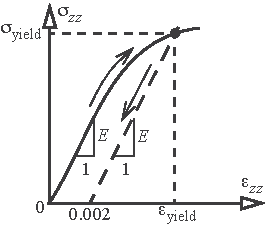
\includegraphics{Figure_4-3.pdf}
\caption{0.2 percent offset yield strength\label{fig4.3}}
\end{wrapfigure}
%}


The yield point, or yield strength, of a material is determined from material characterization tests performed on standard specimens under simple loading situations as specified by the American Society of Testing Methods (ASTM). The standard governing the tensile test of ductile metals is ASTM E8---Standard Test Methods for Tension Testing of Metallic Materials. A plot of the normal stress with respect to the normal strain from typical tensile test of an aluminum alloy is depicted in figure~\ref{fig4.3}. There is an initial linear elastic region whose slope is the modulus of elasticity \textit{E}. Following the linear portion, the slope of the stress-strain curve continuously decreases until a relative maximum engineering stress occurs deep into the response regime where plastic deformation is dominant. For such material behavior we define an \textit{offset yield stress}. A straight line is drawn parallel to the linear elastic portion of the stress-strain curve starting from a strain $\varepsilon_{z z}=\varepsilon_{0.2}=0.002$ on the strain axis. The stress at the intersection of this straight line with the stress-strain curve is defined to be the yield strength $\sigma_{\textrm{yield }}$ of the material. Note that the strain of 0.002, or 0.2 percent (percent strain is defined as $100 \varepsilon_{z z}$), is plastic strain, since unloading the specimen from the point $\left(\varepsilon_{\textrm{yield }}, \sigma_{\textrm{yield}}\right)$ on the stress strain-curve would follow the straight dashed line in figure~\ref{fig4.3} and the strain of 0.002 would not be recovered. However, a permanent strain of 0.2 percent is not considered detrimental for most structural components, and the 0.2 percent offset yield strength has the advantage of being a precisely defined quantity. The offset yield stress is generally the most satisfactory means of defining the yielding event for engineering materials. Metals usually break in tension by the shear stresses acting on planes at $45^{\circ}$ with respect to the tension axis.

Aircraft structural components modeled as thin-walled bars are not only subject to tension, but also compression, bending, and torsion, or a combination of these. Consequently, the material is subject to a combined state of stress. For straight bars with thin-walled cross sections, the dominant stress components are shown in figure~\ref{fig4.2}. These stress components acting on the cross section are directly related to the axial normal force, bending moments, transverse shear forces, and the torque as detailed in article \ref{sec4.1}.

The maximum shear stress criterion and the von Mises criterion were developed to predict yielding for combined stress states in ductile metals (Dowling, 1993). We use von Mises criterion since it compares favorably to test results (Dowling, p. 252) and it is easy to program. The von Mises criterion is based on the shear stress acting on octahedral planes, and it is alternatively called the octahedral shear stress yield criterion. The formula for the von Mises effective stress in thin-walled bar theory is
\begin{align}\label{eq4.31}
\sigma_{\textrm{Mises }}=\sqrt{\sigma_{z}^{2}+3 \sigma_{z s}^{2}}.
\end{align}
If $\sigma_{\textrm{Mises }}<\sigma_{\textrm{yield }}$, then there is no yielding of a ductile metal under a combined stress state, where $\sigma_{\textrm{yield }}$ is determined in the uniaxial tension test. At the initiation of yielding $\sigma_{\textrm{Mises }}=\sigma_{\textrm{yield}}$.

Criteria for failure initiation in modes other than yielding are also formulated in terms of stresses. Examples of stressed-based criteria for failure initiation in fiber-reinforced polymer composites are presented in chapter \ref{ch9}, and the criteria for the initiation crack propagation are presented in chapter \ref{ch13}.

\pagebreak

\section{Structural analyses for extension and flexure}\label{sec4.3}

\subsection{Bending moment diagrams}\label{sec4.3.1}

To determine the axial normal stress distribution in bars subject to lateral loading, we have to first find the distribution of the bending moment. Analyses are presented for a cantilever wing and barge in still water. Airplanes and ships can be regarded as vehicles moving in different mediums, the air or water. In this regard, the study of buoyancy distribution acting on ship structures is instructive in determining the distribution of the bending moment in the hull.

\begin{example}[Cantilever wing with tip tank]\label{ex4.1}\setcounter{equation}{0}\def\theequation{\alph{equation}}%
Consider the cantilever wing with tip tank as shown in figure~\ref{fig4.4}. Given the weight of the tip tank and its contents \textit{W}, the distance $e$ of the weight \textit{W} from the wing tip, the wing span \textit{L}, and the value of the distributed load intensity $f_{r}$ at the wing root, determine the shear force and bending moment along the span.

{\def\thefigure{4.4}
\processfigure[H]{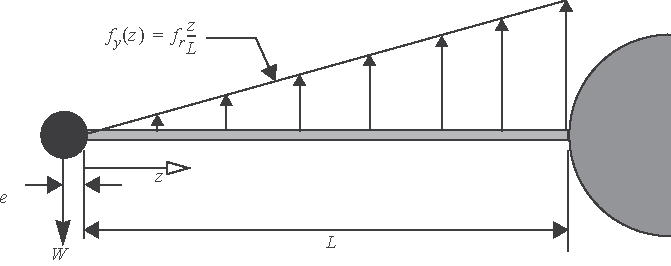
\includegraphics{Figure_4-4.pdf}
}{\caption{Cantilever wing with tip tank.\label{fig4.4}}}}

\noindent\textbf{Solution.}\enspace The differential equilibrium for the shear force is given by eq.~(\ref{eq3.54}) on page \pageref{eq3.54}. Integration of this differential equation from $z =0$ to $z$ results in
\begin{align}\label{ex4.1a}
V_{y}(z)=V_{y}(0)-\int_{0}^{z} f_{r}(u/L) d u,\ \text{which evaluates as}\ V_{y}(z)=V_{y}(0)-f_{r}\left(\frac{z^{2}}{2 L}\right).
\end{align}
The differential equation for the bending moment is given by eq.~(\ref{eq3.55}), where in this example the distributed moment per unit length $m_{x}=0$. Integrating this differential equation from $z =0$ to $z$ results in
\begin{align}\label{ex4.1b}
M_{x}(z)=M_{x}(0)+\int_{0}^{z} V_{y}(u) d u,\ \text{which evaluates as}\ M_{x}(z)=M_{x}(0)+V_{y}(0) z-f_{r}\left(\frac{z^{3}}{6 L}\right).
\end{align}
%{\def\thefigure{4.5}
\begin{wrapfigure}[8]{r}{128pt}
\vspace{-16pt}
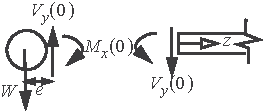
\includegraphics{Figure_4-5.pdf}
\caption{Free body diagram of tip tank\vspace*{10pt}.\label{fig4.5}}
\end{wrapfigure}
%}
 At the wing tip, equilibrium of the tip tank as shown in figure~\ref{fig4.5} leads to
\begin{align}\label{ex4.1c}
V_{y}(0)=W \quad M_{x}(0)=e W.
\end{align}
Hence, the shear force and bending moment are
\begin{align}\label{ex4.1d}
V_{y}(z)=W-f_{r}\left(\frac{z^{2}}{2 L}\right) \quad M_{x}(z)=e W+W z+f_{r}\left(\frac{z^{3}}{6 L}\right) \quad 0 \leq z \leq L.
\end{align}
\vspace*{5pt}
\clearpage

\noindent Take $L=144$~in.~, $e=6\,\textrm{in}.$~, $W=500\,\textrm{lb.}$~, and $f_{r}=70\,\textrm{lb}./\mathrm{in.}$~. Numerical evaluation gives
\begin{align}\label{ex4.1e}
V_{y}(z)=500-(35 z^{2})/144 \quad M_{x}(z)=3,000+500 z-(35 z^{3})/432.
\end{align}
The shear force and bending moment distributions with respect to the normalized coordinate \textit{z/L} are plotted in figure~\ref{fig4.6}

{\def\thefigure{4.6}
\processfigure[H]{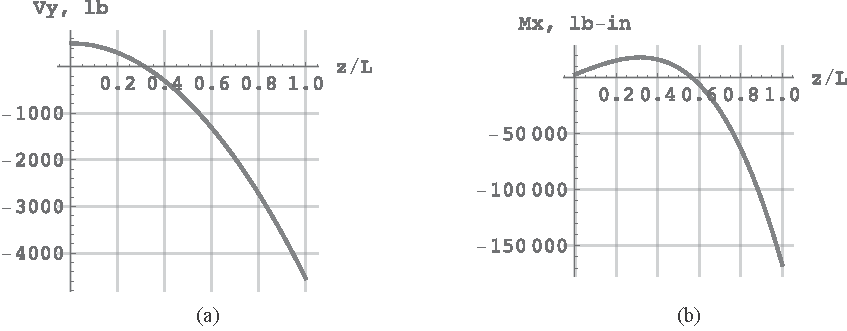
\includegraphics{Figure_4-6.pdf}
}{\caption{(a) Shear force diagram, and (b) Bending moment diagram for example 4.1.\label{fig4.6}}}}


\noindent The shear force equals zero at $z/L=0.315$, which corresponds to $z=45.3557\,\textrm{in}.$. At $z=45.3557\,\textrm{in}.$ the bending moment exhibits a horizontal slope. Thus, the bending moment is a relative maximum at $z=45.3557\,\textrm{in}.$ with a value of 18,118.6\,lb.-in. The largest magnitudes of the shear force and bending moment occur at the wing root where, $V_{y}(L)=-4{,}540\,\textrm{lb.}$ and $M_{x}(L)= -166{,}920$.\,lb.-in.
\end{example}

{\def\thefigure{4.7}
\processfigure[b]{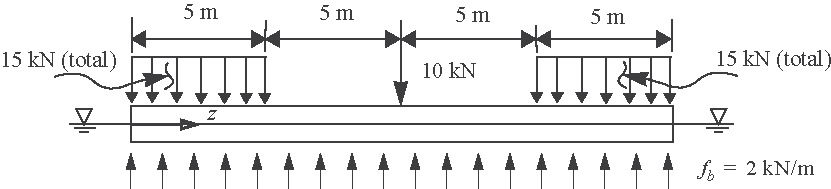
\includegraphics{Figure_4-7.pdf}
}{\caption{Uniform section barge in still water with symmetric load.\label{fig4.7}}\vspace*{20pt}}}

\vspace*{-20pt}

\begin{example*}[Uniform barge with symmetric load]\label{ex4.2}\setcounter{equation}{0}\def\theequation{\alph{equation}}%
Consider a barge at rest in still water with a uniform immersed cross section, and subjected to the symmetrical loads shown in figure~\ref{fig4.7}. There is a distributed load acting on the barge due to buoyancy forces produced by displacing the water. Let $f_{b}$ represent the distributed load intensity due to buoyancy, and $f_{b}$ is a constant along\vadjust{\pagebreak} the barge because the immersed cross section is uniform and the water is still. This is an example of a structure with no boundary supports, and is typical of aerospace and ocean vehicle structures.

\begin{enumerate}[b)]
  \item[a)] Plot the shear force and bending moment diagrams for the barge,
  \item[b)] Determine the maximum axial normal stress.
\end{enumerate}

\noindent\textbf{Solution to part (a).}\enspace Vertical equilibrium of the entire barge requires that the buoyant upthrust equals 40\,kN, so that $f_{b}=2\,\mathrm{KN}/\mathrm{m}$. The total distributed load intensity is the difference between $f_{b}$ and the magnitude of the downward acting applied loading intensity. The point force of 10\,kN acting at $z = 10$\,m is shown schematically in the $f_{y}(z)$-diagram as a downward pointing arrow. Actually, $f_{y} \rightarrow-\infty$ as $z \rightarrow 10~\mathrm{m}$, because a point force is a finite load acting over zero length. Point forces are idealizations to actual loads and introduce discontinuities in the mathematical descriptions of some of the dependent variables.

A semigraphical method is used to sketch the shear force and bending moment diagrams. In this approach we first sketch the distributive load $f_{y}(z)$ (F/L), then the shear force $V_{y}(z)$, and finally the bending moment $M_{x}(z)$. The differential equilibrium equations governing the shear force and the bending moment are eqs. (\ref{eq3.54}) and (\ref{eq3.55}) on page~\pageref{eq3.55}. These equations are repeated in eq. (\textbf{\ref{ex4.2a}}) below.
\begin{align}\label{ex4.2a}
\frac{d V_{y}}{d z}+f_{y}(z)=0 \quad \frac{d M_{x}}{d z}-V_{y}+m_{x}(z)=0.
\end{align}
The prescribed external moment intensity $m_{x}=0$ (F-L/L) in this example. From eq. (\textbf{\ref{ex4.2a}}) we note that the slope of shear diagram at $z$ is the negative of the distributed load intensity at $z$, and that the slope of the moment diagram at $z$ is the shear force at $z$. Integrate eq (\textbf{\ref{ex4.2a}}) with respect to $z$ from $z = z_1$ to $z = z_2$ to get
\begin{align}\label{ex4.2b}
V_{y}\left(z_{2}\right)-V_{y}\left(z_{1}\right)=-\int_{z_{1}}^{z_{2}} f_{y}(z) d z,\ \text{and}\ M_{x}\left(z_{2}\right)-M_{x}\left(z_{1}\right)=\int_{z_{1}}^{z_{2}} V_{y}(z) d z.
\end{align}
Equation (\textbf{\ref{ex4.2b}}) is interpreted in a graphical sense to mean that the difference in the shear force between $z_2$ and $z_1$ is the negative of the area under the distributed loading diagram from $z_1$ to $z_2$, and the difference in the bending moment between $z_2$ and $z_1$ is the area under the shear force diagram from $z_1$ to $z_2$. These are not geometrical areas. The area between the $f_{y}(z)$ curve and the $z$-axis has units of force, and may be positive, zero, or negative.

Free body diagrams of the barge at each end are shown in figure~\ref{fig4.8}. The water pressure varies linearly with the depth of the immersed cross section and acts in $z$-direction. We assume the moment about the $x$-axis caused by the water pressure is small and can be neglected. As the infinitesimal distance $\varepsilon \rightarrow 0$, the distributed loading acting at each end vanishes. In the limit we get the equilibrium conditions
{\def\thefigure{4.8}
\processfigure[H]{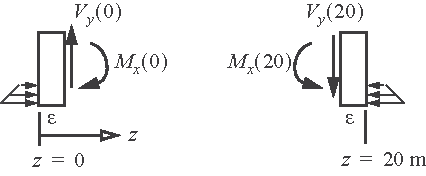
\includegraphics{Figure_4-8.pdf}
}{\caption{Free body diagrams of
the barge at each end. Note $\varepsilon \rightarrow {\textbf{0}}$.\label{fig4.8}}}}
\vspace*{-2\baselineskip}
\begin{align}\label{ex4.2c}
V_{y}(0)=0 \quad M_{x}(0)=0,\ and\ V_{y}(20)=0 \quad M_{x}(20)=0.
\end{align}
\pagebreak
%{\def\thefigure{4.9}
\begin{wrapfigure}[8]{r}{87pt}
%\vspace{-19pt}
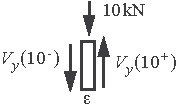
\includegraphics{Figure_4-9.pdf}
\caption{Jump in the shear force.\label{fig4.9}}
\end{wrapfigure}
%}
\noindent From eq. (\textbf{\ref{ex4.2c}}) the shear force\enlargethispage{-1.6\baselineskip} diagram begins at zero, and the slope $d V_{y}/d z$ at $z = 0$ is equal to 1\,kN/m. The slope is constant between $0<z<5 m$, thus ${V}_y(z)$ is a straight line in this range of $z$. The difference in the shear force between $z = 5$\,m and $z = 0$ is equal to the negative of the area under the $f_{y}(z)$ curve, which is 5\,kN. Thus ${V}_y(5) = 5$\,kN since ${V}_y(0) = 0$.  At $z = 5^+$\,m the loading intensity jumps to $+2$\,kN/m. The slope of the shear force jumps from 1\,kN/m to $-2$\,kN/m at $z = 5$~m, but the shear force is itself continuous. The difference $V_y(10) - V_y(5)$ is equal to the negative of the area between the $f_{y}(z)$-curve and the $z$-axis between $z = 5$\,m and $z = 10$\,m. Thus ${V}_y(10) - {V}_y(5) = -10$\,kN, so ${V}_y(10) = -5$\,kN. Note the shear force is zero at $z = 7.5$\,m. At $z = 10$\,m the point force of 10\,kN acts. As shown in figure~\ref{fig4.9}, vertical equilibrium at $z = 10$\,m yields at jump in the shear force ${V}_y(10^+) - {V}_y(10^-) = 10$\,kN, so that ${V}_y(10^+) = 5$\,kN. The slope of the shear at ${z} = 10$\,m is $+2$\,kN/m, and remains constant until $z = 15$\,m. The difference ${V}_y(15) - {V}_y(10^+) = -10$\,kN, so that ${V}_y(15) = -5$\,kN. Finally, the slope changes to $+1$\,kN/m at $z = 15^+$\,m and remains constant in the range $15 < z < 20$. The difference ${V}_y(20) - {V}_y(15) = 5$\,kN, so that ${V}_y(20) = 0$. The shear force equal to zero at $z = 20$\,m is expected from the result in eq. (\textbf{\ref{ex4.2c}}). The shear force diagram is drawn below the loading intensity diagram in figure~\ref{fig4.10}.
{\def\thefigure{4.10}
\processfigure[H]{\vspace*{-12pt}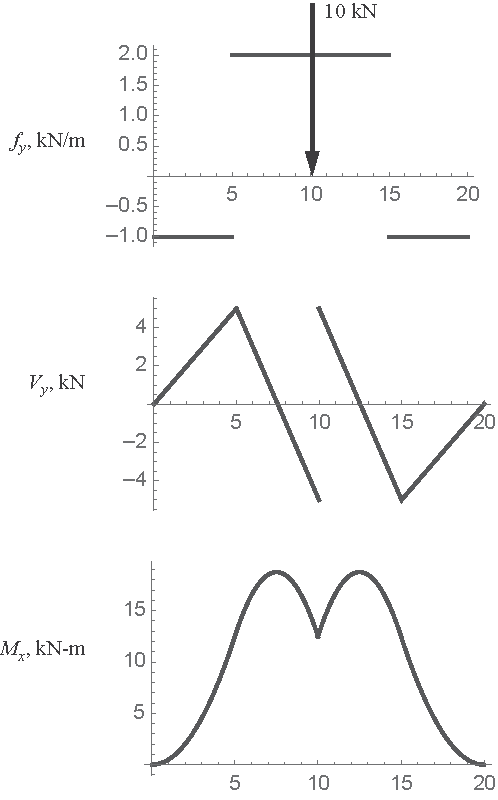
\includegraphics{Figure_4-10.pdf}
}{\caption{The distributed loading, shear force, and bending moment diagrams for the barge in still water.\label{fig4.10}}}}



From eq. (\textbf{c}) the bending moment at $z = 0$ equals zero, and its slope $z = 0$ is equal to zero since the shear force is zero at $\textit{z }= 0$. The slope $d M_{x}/d z$ of the moment diagram increases linearly from zero at $z = 0$ to the 5\,kN, which is the value of the shear force at $z = 5$\,m. The difference $\textit{M}_x(5) - \textit{M}_x(0)$ is equal to the area under shear diagram from $z = 0$ to $z = 5$\,m. Hence, $M_{x}(5) - M_{x}(0) = 12.5$\,kNm, and $M_{x}(5) = 12.5$\,kNm since $M_{x}(0) = 0$. From $z = 5$ to $z = 7.5$ the slope of the moment decreases from 5\,kN to zero. At $z = 7.5, M_{x}$ is a local maximum with a magnitude of 18.75\,kNm. The slope of $M_{x}(z)$ for $7.5 < z < 10$ is negative, decreasing linearly from zero to $-5$\,kN. The difference $M_{x}(10) - M_{x}(7.5) = -6.25$\,kNm, so that $M_{x}(10) = 12.50$\,kNm. The slope of $M_{x}(z)$ at $z = 10$\,m jumps from a $-5$\,kN to $+5$\,kN as shown in figure~\ref{fig4.10}, but the moment itself is continuous. That is, the bending moment exhibits a cusp at $z = 10$\,m. The bending moment diagram in the range $10 < z < 20$ is completed in a manner similar to the description of its construction in the range $0 < z < 10$. In this example the shear force diagram is anti- symmetric about $z = 10$\,m and the bending moment is symmetric about $z = 10$\,m. This follows from the symmetrical loading on the barge.



\noindent\textbf{Solution part (b).}\enspace Let us assume an open cross section of the barge is as shown in figure~\ref{fig4.11}. The thickness of the three branches is 5\,mm, and the section is symmetric about the $y$-axis so the product area moment $I_{x y}=0$. From (\ref{eq4.4}) the cross-sectional coefficients $n_{x}=n_{y}=0$, $k=1$, and $\bar{y}=y$. At $z=7.5~\mathrm{m}$ the shear force is equal to zero and the bending moment has a maximum value of 18.75\,kNm. Hence, the shear stress $\sigma_{z s}=0$ and the axial normal stress (\ref{eq4.6}) is given by
\begin{align}\label{ex4.2d}
\sigma_{z z}=\frac{M_{x}}{I_{x x}} y \quad-\frac{5}{12}~\mathrm{m} \leq y \leq \frac{25}{12}~\mathrm{m},
\end{align}
where the second area moment about the $x$-axis $I_{x x}=(5/128)\,\mathrm{m}^{4}$. The maximum magnitude of the normal stress occurs at $y=(25/12)\,\mathrm{m}$, and it is a tensile stress with the value of
\begin{align}\label{ex4.2e}
\left.\sigma_{z z}\right|_{\max }=\frac{18.75\,\textrm{kNm}(25/12~\mathrm{m})}{(5/128)\,\mathrm{m}^{4}}=1{,}000 \times 10^{3}(\mathrm{N}/\mathrm{m}^{2})=1.0\,\textrm{MPa}.
\end{align}\hfill\qed
\end{example*}

{\def\thefigure{4.11}
\processfigure[H]{\vspace*{-12pt}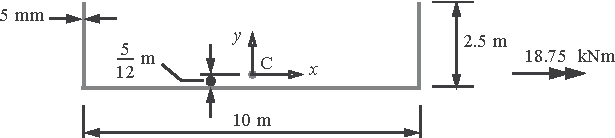
\includegraphics{Figure_4-11.pdf}
}{\caption{Cross section of the barge in example 4.2.\label{fig4.11}}}}


\setcounter{equation}{31}
\subsection{Buoyancy force distribution on ships}\label{sec4.3.2}

The simple uniform buoyancy distribution acting on the barge in example \ref{sec4.2} is an exception to the buoyancy distributions found in practice. It is true that equilibrium requires the total buoyant upthrust to equal the weight of the ship and its contents. However, the distribution of the buoyancy and weight along the length of the ship is not necessarily the same. The difference in the magnitudes of the buoyancy and weight distribution intensities is the applied load intensity $f_{y}(z)$. In ship design three conditions are recognized to compute $f_{y}(z)$ for the same ship. These conditions are called
\begin{itemize}
  \item the still water condition,
  \item the sagging condition, and
  \item the hogging condition.
\end{itemize}
\vspace*{10pt}
\clearpage

A more detailed account of these conditions on the longitudinal bending of the ship is given by Muckle (1967) and Zubaly (1996), and here we only summarize the basic ideas.

A ship in still water is shown in figure~\ref{fig4.12}, and a section A-A between $z$ and $z + \textit{dz}$ is also shown. Archimedes's principle asserts that the buoyant upthrust is equal to the weight of the fluid displaced. Let \textit{A(z)} denote the submerged cross section at $z$, and let $\gamma$ denote the specific weight (force per volume) of the fluid. The differential buoyancy force $dF_{b}$ acting on the ship over a differential length \textit{dz} is
{\def\thefigure{4.12}
\processfigure[H]{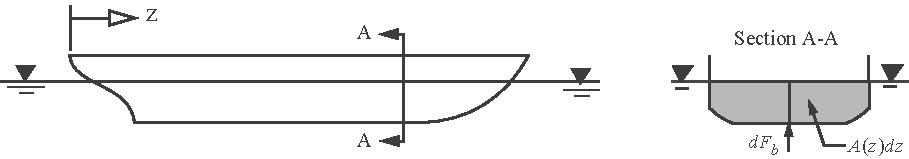
\includegraphics{Figure_4-12.pdf}
}{\caption{A ship in still water.\label{fig4.12}}}}
\vspace*{-2\baselineskip}
\begin{align}\label{eq4.32}
dF_{b}=\gamma A(z) d z.
\end{align}
Consequently, the buoyant upthrust per unit ship length, which we designate $f_{b}$, is equal to $\gamma\textit{A(z)}$; i.e.,
\begin{align}\label{eq4.33}
f_{b}=\frac{d F_{b}}{d z}=\gamma A(z).
\end{align}
\noindent A curve of $f_{b}$ for a ship as well as the weight per unit length is shown in figure~\ref{fig4.13}. Overall equilibrium requires the area under these curves to have the same magnitude. If the submerged cross section is uniform in $z$, as is the case for the barge in example \ref{sec4.2}, the distribution of the buoyancy per unit length $f_{b}$ is a constant.

{\def\thefigure{4.13}
\processfigure[H]{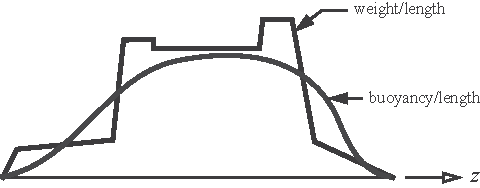
\includegraphics{Figure_4-13.pdf}
}{\caption{Conceptual longitudinal weight and buoyancy distributions acting on a ship.\vspace*{-18pt}\label{fig4.13}}}}

At sea a ship is subject to waves, and this alters the buoyancy distribution. For longitudinal bending of the ship two extreme static conditions are assumed: sagging and hogging. In each condition, the length of the wave is assumed to be the length of the ship. This is an ``accepted'' assumption for the worst buoyancy distribution causing the most severe bending of the ship.

The sagging condition is shown in figure~\ref{fig4.14}(a). The wave crests are at the bow and stern, and the wave trough is amidships. A schematic of the buoyancy per unit length is shown below the ship in figure~\ref{fig4.14}(a). The immersed cross section is the largest at or near the wave crests, and is least near the trough. The intensity of the buoyancy distribution reflects this. In this condition the deck sags and is in compression while the bottom is in tension. The worst location to concentrate the cargo in the ship is amidships, as this will result in the largest bending\break moment.\pagebreak

{\def\thefigure{4.14}
\processfigure[H]{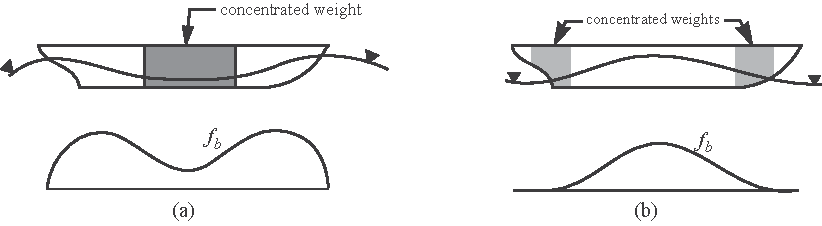
\includegraphics{Figure_4-14.pdf}
}{\caption{Longitudinal bending conditions for a ship. (a) Sagging. (b) Hogging.\vspace*{-12pt}\label{fig4.14}}}}


The hogging condition is depicted in figure~\ref{fig4.14}(b). Here the wave troughs are at bow and stern, and the crest is amidships. The immersed cross section is greatest near amidships and is least near bow and stern. The distribution of the buoyancy per unit length $f_{b}$, shown in figure~\ref{fig4.14}(b), reflects this situation. In hogging the deck is in tension and the bottom is in compression. The worst possible locations to concentrate cargo is fore and aft, as this will produce the greatest bending moment in the ship.


\subsection{Properties of plane areas}\label{sec4.3.3}

First and second area moments of the cross-sectional area need to be determined before evaluating eq.~(\ref{eq4.6}) for the normal stress. Analytical procedures were used in Example \ref{ex3.1} on page \pageref{ex3.1} to compute first and second area moments for a thin-walled bar. Frequently, the composite area technique in conjunction with the parallel axis theorem are used to determine these geometric properties.

\begin{wrapfigure}[14]{L}{137pt}
\vspace{-19pt}
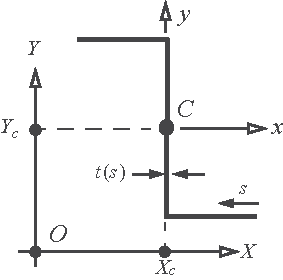
\includegraphics{Figure_4-15.pdf}
\caption{Parallel Cartesian axes systems.\label{fig4.15}}
\end{wrapfigure}
\subsubsection{Parallel axis theorem.} Consider two parallel axes systems in the cross section. The origin of the Cartesian axes $x$ and $y$ coincide with the centroid of the cross-sectional area, which is labeled \textit{C} in figure~\ref{fig4.15}. The second Cartesian system $X$ and $Y$ has its origin at an arbitrary point O, the $X$-axis is parallel to the $x$-axis, and the $Y$-axis is parallel to the $y$-axis. The location of the centroid in the $X$ and $X$ system is denoted by coordinate values $\left(X_{c}, Y_{c}\right)$. Usually the $X$ and $Y$ system is selected as something convenient to start with, and the first and second area moments with respect to the $X$ and $Y$ system are computed or looked up in tables. Then the $\left(X_{c}, Y_{c}\right)$ coordinates of the centroid are computed and the parallel axis theorem is used to find the second area moments in the $x$ and $y$ system.


For a thin-walled bar the area element is $d A=t(s) d s$, in which $s$ denotes the arc-length along the contour $c$, and \textit{t(s)} denotes the thickness of the wall. In general, the thickness may vary smoothly with arc-length, but its magnitude must remain small with respect to the overall dimensions of the cross section. An abrupt change in thickness is modeled by a step change in thickness at a junction. The area of the cross section is given by
\begin{align}\label{eq4.34}
A=\int_{c} t(s) d s.
\end{align}
In the $X$ and $Y$ system, the first area moments are defined as
\begin{align}\label{eq4.35}
Q_{X}=\int_{c} Y t d s \quad Q_{Y}=\int_{c} X t d s.
\end{align}
The relationship between the two parallel coordinate systems is determined from the location of a generic point $s$ on the contour in each system. This relationship is
\begin{align}\label{eq4.36}
X(s)=X_{C}+x(s) \quad Y(s)=Y_{C}+y(s).
\end{align}
If eq.~(\ref{eq4.36}) is substituted into eq.~(\ref{eq4.35}), we get
\begin{align}\label{eq4.37}
Q_{X}=Y_{C} A+Q_{x} \quad Q_{Y}=X_{C} A+Q_{y}.
\end{align}
where
\begin{align}\label{eq4.38}
Q_{x}=\int_{c} y(s) t(s) d s \quad Q_{y}=\int_{c} x(s) t(s) d s.
\end{align}
Since the origin of the $x$ and $y$ system is at the centroid, the first moments $Q_{x}$ and $Q_{y}$ are zero by definition. Setting $Q_{x}=0$ and $Q_{y}=0$ in eq.~(\ref{eq4.37}), we can solve to find the location of the centroid as
\begin{align}\label{eq4.39}
X_{C}=\frac{Q_{Y}}{A} \quad Y_{C}=\frac{Q_{X}}{A}.
\end{align}
In the $X$ and $Y$ coordinate system the second area moments are defined by
\begin{align}\label{eq4.40}
I_{X X}=\int_{c} Y^{2} t d s \quad I_{Y Y}=\int_{c} X^{2} t d s \quad I_{X Y}=\int_{c} X Y t d s.
\end{align}
Second area moments are often called moments of inertia in analogy to moments of inertia of mass elements used in rigid body dynamics. The fact that eq.~(\ref{eq4.40}) is second moments of area elements and not mass elements should be kept in mind even if the terminology ``moments of inertia'' is used in the context of beam bending. Now substitute eq.~(\ref{eq4.36}) for the $X$ and $Y$ coordinates into eq.~(\ref{eq4.40}) to get
\begin{align}\label{eq4.41}
I_{X X}=Y_{C}^{2} A+2 Y_{C} Q_{x}+I_{x x} \quad I_{Y Y}=X_{C}^{2} A+2 X_{C} Q_{y}+I_{y y} \quad I_{X Y}=X_{C} Y_{C} A+X_{C} Q_{x}+Y_{C} Q_{y}+I_{x y},
\end{align}
where the second area moments with respect to the centroid are given by
\begin{align}\label{eq4.42}
I_{x x}=\int_{c} y^{2} t d s \quad I_{y y}=\int_{c} x^{2} t d s \quad I_{x y}=\int_{c} x y t d s.
\end{align}
Since the origin of the $x$ and $y$ coordinates is at the centroid $Q_{x}=Q_{y}=0$, and eq.~(\ref{eq4.41}) reduces to
\begin{align}\label{eq4.43}
I_{X X}=Y_{C}^{2} A+I_{x x} \quad I_{Y Y}=X_{C}^{2} A+I_{y y} \quad I_{X Y}=X_{C} Y_{C} A+I_{x y}.
\end{align}
Equation (\ref{eq4.41}) is the generalized parallel axis theorem, but in problem solving we usually use eq.~(\ref{eq4.39}) to locate the centroid and then the parallel axis theorem reduces to the use of eq.~(\ref{eq4.43}). Note that eq.~(\ref{eq4.42}) shows that $I_{x x}$ and $I_{y y}$ for real areas are always positive in value with dimensional units of ${L^4}$. The product area moment $I_{x y}$ can be positive, zero, or negative in value. The product area moment $I_{x y}$ is zero if either the $x$-axis or $y$-axis is an axis of symmetry of the cross section.

\subsubsection{Radii of gyration.}  Define radii of gyration by
\begin{align}\label{eq4.44}
r_{x x}=\sqrt{I_{x x}/A} \quad r_{y y}=\sqrt{I_{y y}/A}.
\end{align}
The radii of gyration (\ref{eq4.44}) have dimensional units of length. However, the radii of gyration do not locate a physically significant point in the cross section. For example, $r_{X X} \neq Y_{c}+r_{xx}$, where $r_{X X}$ it the radius of gyration with respect to the $X$-axis. (Using the parallel axis theorem, the relation between the radius of gyration about the $X$-axis to the $x$-axis is $r_{X X}^{2}=Y_{C}^{2}+r_{x x}^{2}$.)

\subsubsection{Composite area technique.} The composite area technique for computing the centroid and second area~mom\-ents is a method applicable to cross-sectional areas that can be subdivided into simple geometric shapes whose properties are known. An entire area \textit{A} is subdivided into \textit{N} sub-areas $A_{i}$, $i=1,2, \ldots, N$ as shown in figure~\ref{fig4.16}(a). Known properties of the \textit{i-th} sub-area are its centroid denoted by $C_{i}$, and $A_{i},\left(I_{x x}\right)_{i},\left(I_{y y}\right)_{i},\left(I_{x y}\right)_{i}$. Sub-area coordinate axes are denoted by $\left(x_{i}, y_{t}\right)$ with origin at $C_{i}$. Reference axes are denoted by $(X, Y)$ with origin at point O. The $x_i$-axis is parallel to the \textit{X}-axis, and the $y_i$-axis is parallel to the \textit{Y}-axis. Coordinates $\left(X_{i}, Y_{i}\right)$ in the reference system locate the centroid $C_{i}$ of the \textit{i-th} sub-area.

{\def\thefigure{4.16}
\processfigure[H]{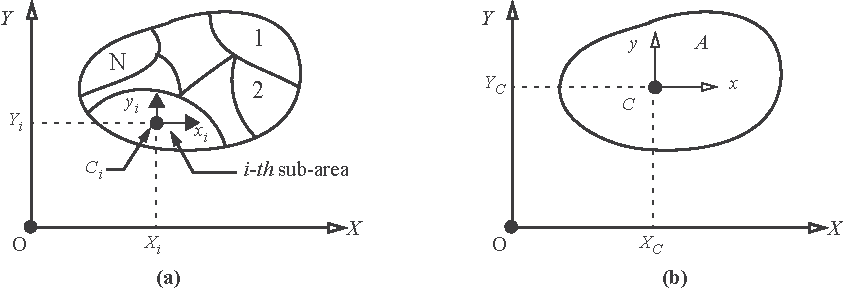
\includegraphics{Figure_4-16.pdf}
}{\caption{(a) Division of area \textit{A} into sub-areas. (b) Assembled properties of area \textit{A}.\label{fig4.16}}}}

The pertinent equations for the assembled area properties are
\begin{align}
\label{eq4.45}
A=\sum^{N}_{i=1,2,\ \ldots} A_{i} \quad A Y_{C} &=\sum^{N}_{i=1,2,\ \ldots} Y_{i} A_{i} \quad A X_{c}=\sum^{N}_{i=1,2,\ \ldots} X_{i} A_{i},\ \text{and}\\
I_{X X}=\sum^{N}_{i=1,2,\ \ldots}(I_{x x}+Y^{2} A)_{i} \quad I_{Y Y}&=\sum^{N}_{i=1,2,\ \ldots}(I_{y y}+X^{2} A)_{i} \quad I_{X Y}=\sum^{N}_{i=1,2,\ \ldots}(I_{x y}+X Y A)_{i}.\label{eq4.46}
\end{align}
The coordinates $\left(X_{C}, Y_{C}\right)$ of the centroid \textit{C} for the entire area shown in figure~\ref{fig4.16}(b) are computed from the last two expressions in eq.~(\ref{eq4.45}). The origin of the parallel coordinate system \textit{x-y} is located at the centroid \textit{C} as shown in figure~\ref{fig4.16}(b). The parallel axis theorem (\ref{eq4.43}) is used to find the second area moments about centroidal system \textit{x-y} after the second area moments in the reference system are determined from eq.~(\ref{eq4.46}).

For branches that can be represented by a thin-walled rectangular area, we can obtain simple formulas for the second area moments. Consider a thin rectangular area, where $0<t \ll b$. The contour is a straight line inclined at a angle $\theta$ as is shown in figure~\ref{fig4.17}. The contour coordinate is denoted by $s$, and the area element is $d A=t d s$. The $x$ and $y$ coordinates of the point $s$ on the contour are given by $x=s \cos \phi$ and $y=s \sin \phi$.

{\def\thefigure{4.17}
\processfigure{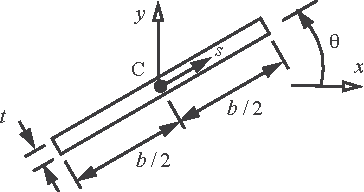
\includegraphics{Figure_4-17.pdf}
}{\caption{Thin rectangular area
inclined at an angle $\theta$.\label{fig4.17}}}}

Hence, the second area moments are computed from
\begin{align}
I_{x x}&=\int\limits^{b/2}_{-b/2}(s \sin \theta)^{2} t d s=\frac{b^{3} t}{12} \sin ^{2} \theta \nonumber\\
\nonumber\\
I_{y y} &=\int\limits^{b/2}_{-b/2}(s \cos \theta)^{2} t d s=\frac{b^{3} t}{12} \cos ^{2} \theta. \label{eq4.47}\\
I_{x y} &=\int\limits^{b/2}_{-b/2}(s \sin \theta)(s \cos \theta) t d s=\frac{b^{3} t}{12} \sin \theta \cos \theta\nonumber
\end{align}

\vspace*{-1\baselineskip}

\begin{example*}[Thin-walled zee section properties by the composite area technique]\label{ex4.3}\setcounter{equation}{0}\def\theequation{\alph{equation}}%
Determine the centroid and the second area moments for the thin-walled zee section shown in figure~\ref{fig4.18}. The section is subdivided into three rectangular branches. One branch corresponds to the web and two branches correspond to the flanges.\vspace*{-6pt}

{\def\thefigure{4.18}
\processfigure[H]{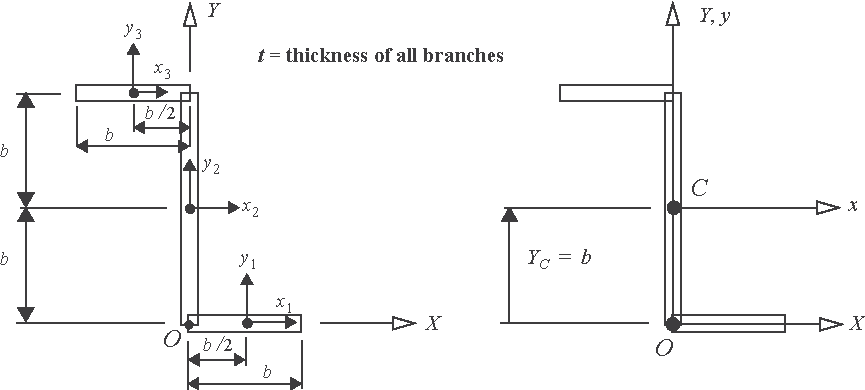
\includegraphics{Figure_4-18.pdf}
}{\caption{Zee section approximated by three rectangular branches.\vspace*{-2\baselineskip}\label{fig4.18}}}}



\noindent\textbf{Solution.}\enspace First we find the centroid. Equation (\ref{eq4.45}) is represented in table \ref{tab4.1} shown below.

Summation of the appropriate columns gives
\begin{align}\label{ex4.3a}
A=4 b t \quad X_{c} A=0 \quad Y_{c} A=4 b^{2} t,
\end{align}
so that the centroid has coordinates $X_{c}=0$ and $Y_{c}=b$.

The second area moments are computed for the reference coordinate system $(X, Y)$ using table \ref{tab4.2} shown below. Note that for the local coordinate systems originating at the centroid in each branch we can identify the angle $\theta$ in eq.~(\ref{eq4.47}) as $\theta_{1}=0^{\circ}$, $\theta_{2}=90^{\circ}$, and $\theta_{3}=0^{\circ}$. These values of the angle $\theta$ in each branch are used to compute the local second area moments in each rectangular branch via eq.~(\ref{eq4.47}).


\begin{table}
\processtable{Areas and first area moments for the zee section\label{tab4.1}}{%
\tabcolsep=17pt\begin{tabular}{@{}llllll@{}}
\toprule
${\boldsymbol i}$ & ${\boldsymbol A}_{\boldsymbol i}$ & ${\boldsymbol X}_{\boldsymbol i}$ & ${\boldsymbol Y}_{\boldsymbol i}$ & ${\boldsymbol X}_{\boldsymbol i} {\boldsymbol A}_{\boldsymbol i}$ & ${\boldsymbol Y}_{\boldsymbol i} {{\boldsymbol A}_{\boldsymbol i}{\textbf{i}}}$\\
\midrule
1 & \textit{bt} & \textit{b/2} & 0 & ${b^2t/2}$ & 0\\
2 & \textit{2bt} & 0 & $b$ & 0 & ${2b^2t}$\\
3 & \textit{bt} & ${- b/2}$ & \textit{2b} & ${- b^2t/2}$ & ${2b^2t}$\\
\midrule
Sum & \textit{4bt} &&& 0 & ${4b^2t}$\\
\botrule
\end{tabular}}{}\vspace*{-10pt}
\end{table}

\begin{table}[!h]\vspace*{6pt}
\processtable{Second area moments for each branch of the zee section\label{tab4.2}}{%
\tabcolsep=8pt\begin{tabular}{@{}lllllll@{}}
\toprule
${\boldsymbol i}$ & {${\boldsymbol Y}_{\boldsymbol i}^{\textbf{2}} {\boldsymbol A}_{\boldsymbol i}$} & {$\textbf{(}{\boldsymbol I}_{{\boldsymbol x}{\boldsymbol x}}\textbf{)}_{\boldsymbol i}$} & ${\boldsymbol X}_{\boldsymbol i}^{\textbf{2}} {\boldsymbol A}_{\boldsymbol i}$ & $\textbf{(}{\boldsymbol I}_{{\boldsymbol y}{\boldsymbol y}}\textbf{)}_{\boldsymbol i}$ & ${\boldsymbol X}_{\boldsymbol i} {\boldsymbol Y}_{\boldsymbol i} {\boldsymbol A}_{\boldsymbol i}$ & $\textbf{(}{\boldsymbol I}_{{\boldsymbol x}{\boldsymbol y}}\textbf{)}_{\boldsymbol i}$\\
\midrule
1& 0& 0& $b^{3}${t/4}& $b^{3}{t/12}$ & 0& 0 \\
2& $(b^{2})2bt$ & ${(2b)}^{3}{t/12}$ & 0& 0& 0& 0 \\
3& ${(2b)}^{2}{bt}$ & 0& $b^{3}{t/4}$ & $b^{3}{t/12}$ & $-b^{3}t$ & 0 \\
\midrule
Sum & ${6b}^{3}t$ & ${2b}^{3}{t/3}$ & $b^{3}{t/2}$ & $b^{3}{t/6}$ & $- b^{3}t$ & 0\\
\botrule
\end{tabular}}{}\vspace*{-10pt}
\end{table}


From the summation of the columns, the second area moments in the $(X, Y)$ system via eq.~(\ref{eq4.46}) are
\begin{equation}\label{ex4.3b}
\begin{gathered}
I_{X X}=6 b^{3} t+2 b^{3} t/3=(20 b^{3} t)/3 \\
I_{Y Y}=(b^{3} t)/2+(b^{3} t)/6=(2 b^{3} t)/3 \\
I_{X Y}=-b^{3} t.
\end{gathered}
\end{equation}
Now we use the parallel axis theorem to transfer these moments to the \textit{x-y} system. Equation (\ref{eq4.43}) gives
\begin{align}
I_{x x}=I_{X X}-Y_{c}^{2} A=\frac{20}{3} b^{3} t-b^{2}(4 b t)=\frac{8}{3} b^{3} t\label{ex4.3c}\\
I_{y y}=I_{Y Y}-X_{c}^{2} A=\frac{2}{3} b^{3} t-(0)(4 b t)=\frac{2}{3} b^{3} t\label{ex4.3d}\\
I_{x y}=I_{X Y}-X_{C} Y_{C} A=-b^{3} t-(0)(b)(4 b t)=-b^{3} t.\label{ex4.3e}
\end{align}\hfill\qed
\end{example*}

\vspace*{-14pt}

\subsection{Neutral axis of the cross section}\label{sec4.3.4}\setcounter{equation}{47}

For the case of a vanishing axial normal force \textit{N}, and neglecting temperature effects, the axial normal stress (\ref{eq4.6}) reduces to
\begin{align}\label{eq4.48}
\sigma_{z z}=\frac{k M_{x}}{I_{x x}} \bar{y}+\frac{k M_{y}}{I_{y y}} \bar{x}=\frac{k M_{x}}{I_{x x}}\left(y-n_{y} x\right)+\frac{k M_{y}}{I_{y y}}\left(x-n_{x} y\right)=k\left(\frac{-n_{y} M_{x}}{I_{x x}}+\frac{M_{y}}{I_{y y}}\right) x+k\left(\frac{M_{x}}{I_{x x}}-\frac{n_{x} M_{y}}{I_{y y}}\right) y.
\end{align}
\vspace*{4pt}
\clearpage

\noindent At the centroid where $x=y=0$ the axial normal stress vanishes. Set the axial normal stress equal to zero to get
\begin{align}\label{eq4.49}
\left(\frac{-n_{y} M_{x}}{I_{x x}}+\frac{M_{y}}{I_{y y}}\right) x+\left(\frac{M_{x}}{I_{x x}}-\frac{n_{x} M_{y}}{I_{y y}}\right) y=0.
\end{align}
Equation (\ref{eq4.49}) defines a straight line in the cross section that is called the neutral axis. Substitute the definitions of $n_{x}$ and $n_{y}$ from eq.~(\ref{eq4.4}) into eq.~(\ref{eq4.49}), and then solve for $y$ in terms of $x$. Let these coordinates be denoted as $\left(x_{\mathrm{NA}}, y_{\mathrm{NA}}\right)$. After some algebra we find
\begin{align}\label{eq4.50}
y_{\mathrm{NA}}=-\left(\frac{-I_{x y} M_{x}+I_{x x} M_{y}}{I_{y y} M_{x}-I_{x y} M_{y}}\right) x_{\mathrm{NA}}=-(\tan \beta) x_{\mathrm{NA}},
\end{align}
where
\begin{align}\label{eq4.51}
\tan \beta=\frac{-I_{x y} M_{x}+I_{x x} M_{y}}{I_{y y} M_{x}-I_{x y} M_{y}}.
\end{align}

\vspace*{-5pt}

\begin{example}[Normal stress distribution in a cantilever beam subject to pure bending]\label{ex4.4}\setcounter{equation}{0}\def\theequation{\alph{equation}}%
The cantilever beam shown in figure~\ref{fig4.19} is subject to a bending moment \textit{M} at its tip. The cross section is the thin-walled zee shown in figure~\ref{fig4.18}. The second area moments about the centroidal axes are given by eqs. (\textbf{\ref{ex4.4c}}) to (\textbf{\ref{ex4.4e}}) in example \ref{fig4.3}. Determine the neutral axis in the cross section and the distribution of the bending normal stress.

{\def\thefigure{4.19}
\processfigure[H]{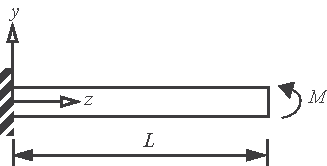
\includegraphics{Figure_4-19.pdf}
}{\caption{Pure bending of a cantilever beam with a zee cross section.\label{fig4.19}}}}

\vspace*{-1\baselineskip}
\noindent\textbf{Solution.}\enspace First, note that the components of the prescribed bending moment are $M_{x}=-M$ and $M_{y}=0$. Thus, the cantilever beam is subject to loading in the \textit{y-z} plane. The equation of the neutral axis is $y_{\mathrm{NA}}=-(\tan \beta) x_{\mathrm{NA}}$, where eq.~(\ref{eq4.51}) is
\begin{align}\label{ex4.4a}
\tan \beta=\frac{(-I_{x y})(-M)}{I_{y y}(-M)}=\frac{-(-b^{3} t)}{\displaystyle\frac{2}{3} b^{3} t}=\displaystyle\frac{3}{2}.
\end{align}
The angle $\beta=56.31^{\circ}$.

To compute the distribution of the normal stress (\ref{eq4.6}) in the cross section, we begin by evaluating section coefficients (\ref{eq4.4}):
\begin{align}\label{ex4.4b}
n_{x}=I_{x y}/I_{x x}=-3/8 \quad n_{y}=I_{x y}/I_{y y}=-3/2 \quad k=\frac{1}{1-n_{x} n_{y}}=16/7.
\end{align}
The coordinates in each branch of the cross section defined by eq.~(\ref{eq4.7}) are
\begin{align}\label{ex4.4c}
\bar{x}_{i}(s)=x_{i}(s)-n_{x} y_{i}(s) \quad \bar{y}_{i}(s)=y_{i}(s)-n_{y} x_{i}(s) \quad i=1,2,3.
\end{align}\pagebreak
The normal stress (\ref{eq4.6}) in \textit{i-th} branch is given by
\begin{align}\label{ex4.4d}
\left(\sigma_{z z}\right)_{i}=\left[\frac{k(-M)}{I_{x x}}\right] \bar{y}_{i}(s)=\left[\frac{k(-M)}{I_{x x}}\right]\left(y_{i}-n_{y} x_{i}\right)=\frac{6}{7 b^{3} t}(-M)\left(y_{i}+\frac{3}{2} x_{i}\right).
\end{align}
Coordinates in branch 1 are $\left(x_{1}, y_{1}\right)=\left(x_{1},-b\right)$, in branch 2 $\left(x_{2}, y_{2}\right)=\left(0, y_{2}\right)$, and in branch 3 $\left(x_{3}, y_{3}\right)=\left(x_{3}, b\right)$. The normal stress in each branch is a linear function of the contour coordinate. The results are
\begin{gather}
\left(\sigma_{z z}\right)_{1}=\frac{6}{7 b^{3} t}(-M)\left(-b+\frac{3}{2} x_{1}\right) \quad 0 \leq x_{1} \leq b,\label{ex4.4e}\\[6pt]
\left(\sigma_{z z}\right)_{2}=\frac{6}{7 b^{3} t}(-M)\left(y_{2}-n_{y} x_{2}\right)=\frac{6}{7 b^{3} t}(-M) y_{2} \quad-b \leq y_{2} \leq b,\ \text{and}\label{ex4.4f}\\[6pt]
\left(\sigma_{z z}\right)_{3}=\frac{6}{7 b^{3} t}(-M)\left(y_{3}-n_{y} x_{3}\right)=\frac{6}{7 b^{3} t}(-M)\left(b+\frac{3}{2} x_{3}\right) \quad-b \leq x_{3} \leq 0.\label{ex4.4g}
\end{gather}
The neutral axis and the bending normal stress distribution are shown in figure~\ref{fig4.20}.
\end{example}



{\def\thefigure{4.20}
\processfigure[H]{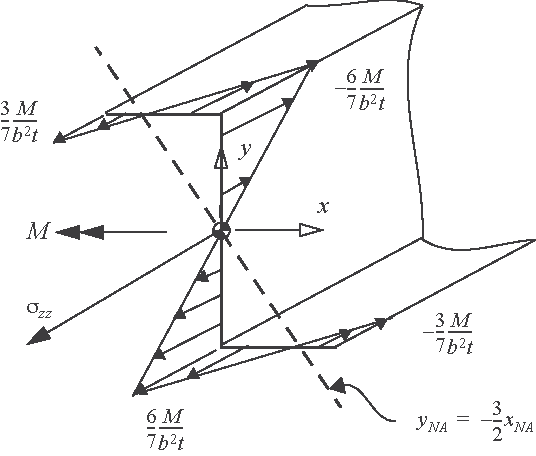
\includegraphics{Figure_4-20.pdf}
}{\caption{Bending normal stress distribution along the contour of the zee section.\label{fig4.20}}}}

\vspace*{-10pt}

\begin{example}[Displacements of the cantilever beam of example \ref{ex4.4}]\label{ex4.5}\setcounter{equation}{0}\def\theequation{\alph{equation}}%
Determine the lateral displacement functions $u(z)$ and $v(z)$, $0 \leq z \leq L$, for the zee section beam of~ex\-ample \ref{ex4.4}.

\noindent\textbf{Solution.}\enspace First note that this a statically determinate beam subject to pure bending. The equilibrium equations are satisfied for $M_{x}=-M$ and $M_{y}=0$ for all $z \in(0, L)$, where \textit{M} denotes the specified end moment. To find the lateral displacements $u(z)$ and $v(z)$, $0 \leq z \leq L$, we begin with matrix eq.~(\ref{eq4.1}), which for this example\break reduces\vspace*{10pt} to\pagebreak
\begin{align}\label{ex4.5a}
\left[\begin{array}{@{}l@{}}d w/d z \\[3pt]d \phi_{x}/d z \\[3pt]d \phi_{y}/d z\end{array}\right]=\frac{1}{E}\left[\begin{array}{@{}ccc@{}}1/A & 0 & 0 \\[3pt]0 & k/I_{x x} & \left(-k n_{x}\right)/I_{y y} \\[3pt]0 & \left(-k n_{y}\right)/I_{x x} & k/I_{y y}\end{array}\right]\left[\begin{array}{@{}c@{}}0 \\[3pt]-M \\[3pt]0\end{array}\right].
\end{align}
For this pure bending case the derivatives of the rotations are given by
\begin{gather}
\frac{d \phi_{x}}{d z}=\frac{k(-M)}{E I_{x x}}=\frac{16/7}{(8/3) E b^{3} t}(-M)=-\frac{6}{7}\left(\frac{M}{E b^{3} t}\right),\ \text{and}\label{ex4.5b}\\[6pt]
\frac{d \phi_{y}}{d z}=-\frac{k n_{y}}{E I_{x x}}(-M)=-\frac{(16/7)(-3/2)}{(8/3) E b^{3} t}(-M)=-\frac{9}{14}\left(\frac{M}{E b^{3} t}\right).\label{ex4.5c}
\end{gather}
Integrate eqs. (\textbf{\ref{ex4.5b}}) and (\textbf{\ref{ex4.5c}}) from $z = 0$ to $z$ to get
\begin{gather}
\phi_{x}(z)-\phi_{x}(0)=\int_{0}^{z}\left[-\frac{6}{7}\left(\frac{M}{E b^{3} t}\right)\right] d z=\left[-\frac{6}{7}\left(\frac{M}{E b^{3} t}\right)\right] z,\ \text{and}\label{ex4.5d}\\[6pt]
\phi_{y}(z)-\phi_{y}(0)=\int_{0}^{z}\left[-\frac{9}{14}\left(\frac{M}{E b^{3} t}\right)\right] d z=\left[-\frac{9}{14}\left(\frac{M}{E b^{3} t}\right)\right] z.\label{ex4.5e}
\end{gather}
At $z = $0 the beam is clamped to the rigid wall so that the rotations of the cross section at the wall are $\phi_{x}(0)=\phi_{y}(0)=0$. The results for the rotations are
\begin{align}\label{ex4.5f}
\phi_{x}(z)=-\frac{6}{7}\left(\frac{M}{E b^{3} t}\right) z \quad \phi_{y}(z)=-\frac{9}{14}\left(\frac{M}{E b^{3} t}\right) z.
\end{align}
The cantilever beam is subject to pure bending and by equilibrium the transverse shear forces $V_{x}=V_{y}=0$, for $0 \leq z \leq L$. Hooke's law (\ref{eq4.27}) then yields that the transverse shear strains $\psi_{x}=\psi_{y}=0$, for $0 \leq z \leq L$. Vanishing of the transverse shear strains in eq.~(\ref{eq4.28}) leads to
\begin{align}\label{ex4.5g}
\psi_{x}=\frac{d u}{d z}+\phi_{y}=0 \quad \psi_{y}=\frac{d v}{d z}+\phi_{x}=0.
\end{align}
From eqs. (\textbf{f}) and (\textbf{g}) the derivatives of the displacements are given by
\begin{align}\label{ex4.5h}
\frac{d u}{d z}=-\phi_{y}=\frac{9}{14}\left(\frac{M}{E b^{3} t}\right) z \quad \frac{d v}{d z}=-\phi_{x}=\frac{6}{7}\left(\frac{M}{E b^{3} t}\right) z.
\end{align}
Integrate eq. (\textbf{h}) from $z=0$ to $z$ to get
\begin{align}\label{ex4.5i}
u(z)-u(0)=\frac{9}{14}\left(\frac{M}{E b^{3} t}\right) \frac{z^{2}}{2} \quad v(z)-v(0)=\frac{6}{7}\left(\frac{M}{E b^{3} t}\right) \frac{z^{2}}{2}.
\end{align}
At the clamped end the beam displacements equal zero. Thus, the displacements are
\begin{align}\label{ex4.5j}
\left.u(z)=\frac{9}{14}\left(\frac{M}{E b^{3} t}\right) \frac{z^{2}}{2} \quad v(z)=\frac{6}{7} \frac{M}{E b^{3} t}\right) \frac{z^{2}}{2}.
\end{align}
The view of the lateral displacements of the beam at $z=L$ are shown in figure~\ref{fig4.21}. As a result of $I_{x y} \neq 0$ the beam displaces both vertically and horizontally for a load that is applied in \textit{y-z} plane.
\end{example}

{\def\thefigure{4.21}
\begin{figure}
\centering{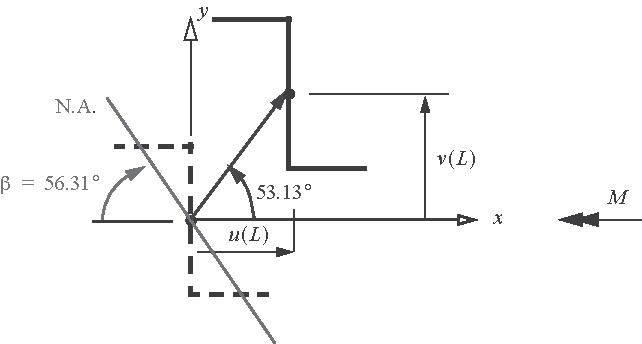
\includegraphics{Figure_4-21.pdf}}
\caption{Displacement of the centroid at the tip of the cantilever beam subject to pure bending.\label{fig4.21}} \end{figure}
}

\begin{example}[Transverse bending of a cantilever beam]\label{ex4.6}\setcounter{equation}{0}\def\theequation{\alph{equation}}%
Consider a uniform cantilever beam from example \ref{ex4.4} subject to a vertical force \textit{F} acting through the shear center at its free end as shown in figure~\ref{fig4.22}. There is no change in temperature from the stress-free state. The cross section is the thin-walled zee shown in figure~\ref{fig4.18}. Determine the displacements of the cantilever.

{\def\thefigure{4.22}
\processfigure[H]{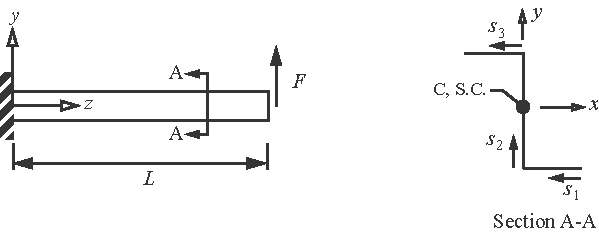
\includegraphics{Figure_4-22.pdf}
}{\caption{Transverse bending\break of a cantilever beam with a zee cross section.\label{fig4.22}}}}

\vspace*{-1\baselineskip}
\noindent\textbf{Solution.}\enspace The cantilever is statically determinate, and from equilibrium the shear force and bending moment are
\begin{align}\label{ex4.6a}
V_{y}=F \quad M_{x}=-(L-z) F \quad 0 \leq z \leq L.
\end{align}
From Hooke's law (\ref{eq4.1}) we find the derivatives of the rotations are
\begin{align}\label{ex4.6b}
\frac{d \phi_{x}}{d z}=\frac{k M_{x}}{E I_{x x}}=\frac{-k}{E I_{x x}}(L-z) F \quad \frac{d \phi_{y}}{d z}=-\frac{k n_{y}}{E I_{x x}} M_{x}=\frac{k n_{y}}{E I_{x x}}(L-z) F.
\end{align}
Integrate the rotations in eq. (\textbf{b}) with respect to coordinate $z$ and impose $\phi_{x}(0)=\phi_{y}(0)=0$ at the clamped end of the cantilever to get
\begin{align}\label{ex4.6c}
\phi_{x}=\frac{-3 z(2 L-z)}{7 E b^{3} t} F \quad \phi_{y}=\frac{-9 z(2 L-z)}{14 b^{3} t E} F.
\end{align}
From eq.~(\ref{eq4.27}) the shear strains of the cantilever beam are
\begin{align}\label{ex4.6d}
\psi_{x}=c_{x y} F \quad \psi_{y}=c_{y y} F.
\end{align}
The compliance coefficients (\ref{eq4.29}) for this example are
\begin{align}
c_{x y}=\frac{k^{2}}{I_{x x} I_{y y}}\left[\int\limits_{0}^{b} \bar{Q}_{x 1} \bar{Q}_{y 1} d s_{1}+\int\limits_{0}^{2b} \bar{Q}_{x 2} \bar{Q}_{y 2} d s_{2}+\int\limits_{0}^{b} \bar{Q}_{x 3} \bar{Q}_{y 3} d s_{3}\right] \frac{1}{G t},\ \text{and}\label{ex4.6e}\\
c_{y y}=\left(\frac{k}{I_{x x}}\right)^{2}\left[\int\limits_{0}^{b} \bar{Q}_{x 1}^{2} d s_{1}+\int\limits_{0}^{2b} \bar{Q}_{x 2}^{2} d s_{2}+\int\limits_{0}^{b} \bar{Q}_{x 3}^{2} d s_{3}\right] \frac{1}{G t}.\label{ex4.6f}
\end{align}
To evaluate the compliance coefficients in eq. (\textbf{\ref{ex4.6d}}) we need the parametric equations of the contour of the cross section with respect to centroidal coordinates. The equations are listed in table \ref{tab4.3}.

\begin{table}[h]\vspace*{4pt}
\processtable{Contour coordinate functions\label{tab4.3}}{%
\tabcolsep=10pt\begin{tabular}{@{}llll@{}}
\toprule
\colhead{Branch} & \colhead{$x_{i}\left(s_{i}\right)$} & \colhead{$y_{i}\left(s_{i}\right)$} & \\
\midrule
$i = 1$ & $b-s_{1}$ & $-b$ & $0 \leq s_{1} \leq b$\\
$i = 2$ & 0 & $-b+s_{2}$ & $0 \leq s_{2} \leq 2 b$\\
$i = 3$ & $-s_{3}$ & $b$ & $0 \leq s_{s} \leq b$\\
\botrule
\end{tabular}}{}\vspace*{-10pt}
\end{table}

We need to determine the distribution functions $\bar{Q}_{x i}\left(s_{i}\right)$ and $\bar{Q}_{y i}\left(s_{i}\right)$, $i=1,2,3$, beginning with the contour origin from the general expression in eq.~(\ref{eq4.9}). The contour origin is in branch 1 where $s_{1}=0$ at its intersection with the traction-free longitudinal edge. As we move along the contour each branch is cut at a generic value of its contour coordinate. The area of the contour preceding the cut determines the range of integration for the distribution function as shown in figure~\ref{fig4.23}. Using the parametric equations in table \ref{tab4.3} the results for branch one are
\begin{align}
\bar{Q}_{x 1}\left(s_{1}\right)&=\int_{0}^{s_{1}}\left[y_{1}\left(s_{1}\right)-n_{y} x_{1}\left(s_{1}\right)\right] t d s_{1}=\frac{1}{4}\left(2 b-3 s_{1}\right) s_{1} t,\ \text{and}\nonumber\\
\bar{Q}_{y 1}\left(s_{1}\right)&=\int_{0}^{s_{1}}\left[x_{1}\left(s_{1}\right)-n_{x} y_{1}\left(s_{1}\right)\right] t d s_{1}=\frac{1}{8}\left(5 b-4 s_{1}\right) s_{1} t.\label{ex4.6g}
\end{align}
\noindent For a cut in branch 2, the integration includes all of branch 1 and the integration of the segment in branch 2. The distribution functions for the cut in branch 2 are\vspace*{-1\baselineskip}
{\def\thefigure{4.23}
\processfigure[b]{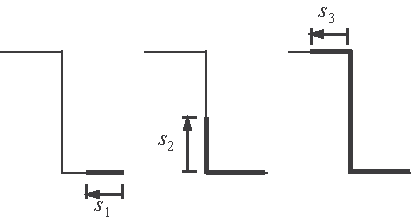
\includegraphics{Figure_4-23.pdf}
}{\caption{Range of integration along the contour to compute the distribution functions.\label{fig4.23}}}}
\pagebreak
\begin{gather}
\bar{Q}_{x 2}\left(s_{2}\right)=\bar{Q}_{x 1}(b)+\int_{0}^{s_{2}}\left[y_{2}\left(s_{2}\right)-n_{y} x_{2}(s_{2})\right] t d s_{2}=-\frac{1}{4}(b^{2}+4 b s_{2}-2 s_{2}^{2}) t,\ \text{and}\label{ex4.6h}\\
\bar{Q}_{y 2}\left(s_{2}\right)=\bar{Q}_{y 1}(b)+\int_{0}^{s_{2}}\left[x_{2}\left(s_{2}\right)-n_{x} y_{2}\left(s_{2}\right)\right] t d s_{2}=\frac{1}{16}(2 b^{2}-6 b s_{2}+3 s_{2}^{2}) t,\,\textrm{where } 0 \leq s_{2} \leq 2 b.\label{ex4.6i}
\end{gather}
For a cut in branch 3, the integration includes all of branch 1, all of branch 2, and the integration of the segment in branch 3. The distribution functions for the cut in branch 3\vspace*{-2pt} are
\begin{gather}
\bar{Q}_{x 3}\left(s_{3}\right)=\bar{Q}_{x 2}(2 b)+\int_{0}^{s_{3}}\left[y_{3}\left(s_{3}\right)-n_{y} x_{3}\left(s_{3}\right)\right] t d s_{3}=-\frac{1}{4}(b^{2}-4 b s_{3}+3 s_{3}^{2}) t,\ \text{and}\label{ex4.6j}\\
\bar{Q}_{y 3}\left(s_{3}\right)=\bar{Q}_{y 2}(2 b)+\int_{0}^{s_{3}}\left[x_{3}\left(s_{3}\right)-n_{x} y_{3}\left(s_{3}\right)\right] t d s_{3}=\frac{1}{8}(b^{2}+3 b s_{3}-4 s_{3}^{2}) t,\ \text{where}\ 0 \leq s_{3} \leq b.\label{ex4.6k}
\end{gather}
Substitute the distribution functions in eqs. (\textbf{\ref{ex4.6g}}) to (\textbf{\ref{ex4.6k}}) into the compliance coefficients of eqs. (\textbf{\ref{ex4.6e}}) and (\textbf{\ref{ex4.6f}}), followed by integration, to\vspace*{-2pt} find
\begin{align}
c_{x y}=\frac{9}{196 b G t} \quad c_{y y}=\frac{267}{490 b G t}.\label{ex4.6l}
\end{align}
From the definition of the shear strains (\ref{eq4.28}), we get the following integrals for the displacements that satisfy the boundary conditions $u(0)=v(0)=0$\vspace*{-2pt}:
\begin{align}\label{ex4.6m}
u(z)=\int_{0}^{z}\left(\psi_{x}-\phi_{y}\right) d z \quad v(z)=\int_{0}^{z}\left(\psi_{y}-\phi_{x}\right) d z.
\end{align}
Substitute the compliance coefficients from eq. (\textbf{\ref{ex4.6i}}) into Hooke's law (\textbf{\ref{ex4.6d}}), followed by substituting the result for shear strains into eq. (\textbf{\ref{ex4.6m}}). Then substitute eq. (\textbf{\ref{ex4.6c}}) for the rotations into eq. (\textbf{\ref{ex4.6m}}). Perform the integration with respect to $z$ to get\vspace*{-2pt}:
\begin{align}\label{ex4.6n}
u(z)=\frac{9 F z}{196 b G t}+\frac{9 L F z^{2}}{14 b^{3} t E}-\frac{3 F z^{3}}{14 b^{3} t E} \quad v(z)=\frac{267 F z}{480 b t G}+\frac{3 L F z^{2}}{7 b^{3} t E}-\frac{F z^{3}}{7 b^{3} t E}.
\end{align}
The vertical displacement at point of application of the force \textit{F}\vspace*{-2pt} is
\begin{align}\label{ex4.6o}
v(L)=\left(\frac{2 L^{3}}{7 b^{3} t E}+\frac{267 L}{490 b t G}\right) F=\left(\frac{3 L^{3} F}{7 b^{3} t E}\right)\left[1+\frac{267 b^{2}}{140 L^{2}} \frac{E}{G}\right],
\end{align}
where the last result was obtained by factoring out the first term on the right-hand side. For aluminum alloys $E/G \approx 2.5$, eq. (\textbf{\ref{ex4.6o}}) can be manipulated to the\vspace*{-2pt} form
\begin{align}\label{ex4.6p}
v(L)=\frac{16 L^{3} F}{21 E I_{x x}} \underbrace{\left[1+\frac{4.77}{(L/b)^{2}}\right]}_{=\,g(L/b)}.
\end{align}
The function $g(L/b)$ is evaluated for several ratios of $L/b$, and the results are listed in table \ref{tab4.4}. The function $g(L/b) \rightarrow 1$ for values of $L/b>10$, which implies the displacement $v(L) \rightarrow \frac{16 L^{3} F}{21 E I_{x x}}$ for $L/b>10$.

This result means the contribution of the displacement due to transverse shear deformation is negligible with respect to the component due to bending for beams that are long with respect to their cross-sectional dimensions. To neglect the influence of transverse shear means we can set shear strains $\psi_{x}=0$ and $\psi_{y}=0$. Setting the shear strains equal to zero in Hooke's law for transverse shear in (\ref{eq4.27}) means the shear forces equal zero. However, the shear forces are necessary for beam equilibrium. Hence, we omit Hooke's law for transverse shear in a theory where the shear strains are assumed equal to zero. The beam theory neglecting transverse shear strains is called the \textbf{Euler-Bernoulli} beam theory.
\end{example}
\clearpage

\begin{table}
\processtable{Ratio of the transverse shear\break
 displacement to the bending displacement\label{tab4.4}}{%
\tabcolsep=70pt\begin{tabular}{@{}ll@{}}
\toprule
\colhead{$L/b$} & \colhead{$g(L/b)$} \\
\midrule
1 & 5.77\\
2 & 2.19\\
5 & 1.19\\
10 & 1.05\\
15 & 1.02\\
\botrule
\end{tabular}}{\vspace*{-13pt}}
\end{table}

\section{Structural analyses for transverse shear and torsion}\label{sec4.4}
The shear stress $\sigma_{z s}$ is directly proportional to the transverse shear force components $V_x$ and ${V}_y$, and the torque ${M}_z$ for a straight bar and for infinitesimal deformations of a Hookean material. Procedures to calculate $\sigma_{z s}$ are different for an open contour and for a closed contour. The stress analysis for an open cross-sectional contour is presented in example \ref{ex4.7}, and the stress analysis for a closed cross-sectional contour is presented in example \ref{ex4.8}.

\enlargethispage{1\baselineskip}

\begin{example*}[Shear stress analysis for an open cross-sectional contour\label{ex4.7}]\setcounter{equation}{0}\def\theequation{\alph{equation}}The open contour shown in figure~\ref{fig4.24} consists of a semicircular branch of radius $a$. \begin{wrapfigure}[11]{R}{150pt}
\vspace{-19pt}
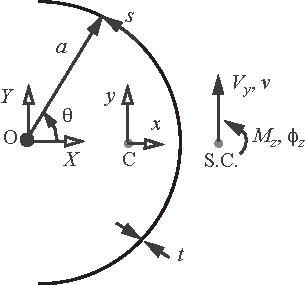
\includegraphics{Figure_4-24.pdf}
\caption{Semicircular, open section.\label{fig4.24}}
\end{wrapfigure} For simplicity the origin of the \textit{X-Y} system is at the center of the semicircle which is labeled point O in figure~\ref{fig4.24}. The \textit{X}-axis is an axis of symmetry, and the centroid C and shear center S.C. lie on this axis. To find the shear center we take the shear force $V_{x}=0$. The shear force $V_{y}$ and the torque $M_{z}$ act at the shear center. If $M_{z}=0$, then the shear force ${V}_y$ causes a displacement $\nu$ in bending of the bar, and $\phi_{z}=0$. If $V_{y}=0$, then the torque $M_{z}$ causes a rotation $\phi_{z}$ twisting the bar, and $v=0$ at the shear center.

Determine
\begin{enumerate}[b)]
  \item[a)] the location of the centroid,
  \item[b)] the shear flow due $V_{y}$,
  \item[c)] the location of the shear center, and
  \item[d)] the shear stress $\sigma_{z s}$ in terms of $V_{y}$ and $M_{z}$.
\end{enumerate}




\subsubsection{Solution to part (a).} The parametric equations of the semicircular contour are
\begin{align}\label{ex4.7a}
X(\theta)=a \cos \theta \quad Y(\theta)=a \sin \theta \quad s=a \theta \quad-\pi/2 \leq \theta \leq \pi/2.\end{align}
We compute the area \textit{A}, the first area moment about the \textit{Y}-axis $Q_{Y}$, and the location of the centroid as follows.
\begin{align}\label{ex4.7b}
A=\int_{-\pi/2}^{\pi/2} t a d \theta=a \pi t \quad Q_{Y}=\int_{-\pi/2}^{\pi/2} X(\theta) t a d \theta=2 a^{2} t \quad X_{C}=Q_{Y}/A=2 a/\pi.
\end{align}
\vspace*{-16pt}
\clearpage
\noindent The coordinates relative to the centroid, and the second area moment about the $x$-axis through the centroid are
\begin{align}\label{ex4.7c}
x(\theta)=X(\theta)-X_{C}=a \cos \theta-2 a/\pi \quad y(\theta)=Y(\theta) \quad I_{x x}=\int_{-\pi/2}^{\pi/2} y^{2}(\theta) t a d \theta=a^{3} \pi t/2.
\end{align}

\vspace*{-5pt}

\subsubsection{Solution to part (b).} The distribution function for the shear flow with the contour origin at $\theta=-\pi/ 2$ is given by
\begin{align}\label{ex4.7d}
Q_{x}(\theta)=\int_{-\pi/2}^{\theta} y(\theta) \textit{tad} \theta=-a^{2} t \cos \theta \quad-\pi/2 \leq \theta \leq \pi/2.\end{align}
Since the product area moment $I_{x y}=0$, eq.~(\ref{eq4.4}) yields the parameters $n_{x}=n_{y}=0$ and $k=1$. The shear flow in eq.~(\ref{eq4.13}) on page~\pageref{eq4.13} reduces to
\begin{align}\label{ex4.7e}
q(s, z)=-\frac{V_{y}}{I_{x x}} Q_{x}(s),\end{align}
and the explicit equation for the shear flow is
\begin{align}\label{ex4.7f}
q(\theta)=-V_{y} Q_{x}(\theta)/I_{x x}=\frac{2 V_{y}}{(a \pi)} \cos \theta.\end{align}
The shear flow is plotted normal to the contour in figure~\ref{fig4.25}, and it apparent in the figure that the shear flow is a maximum at $\theta = 0$.


\begin{wrapfigure}[13]{L}{78pt}
\vspace{-24pt}
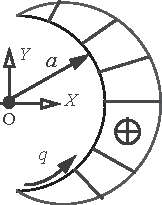
\includegraphics{Figure_4-25.pdf}
\caption{Distribution of the shear flow in the open section. $V_{y} > \textbf{0}$.\label{fig4.25}}
\end{wrapfigure}
\subsubsection{Solution to part (c).}

The coordinates of the shear center relative to the centroid is given in eq.~(\ref{eq4.8}) on page \pageref{eq4.8}. In this example the equation for the coordinate $x_{S c}$ reduces to
\begin{align}\label{ex4.7g}
x_{s c}=-\left(\frac{1}{I_{x x}}\right)\left[\int_{c} r_{n c}(\theta) Q_{x}(\theta) a d \theta \mid\right.\!,\end{align}
\noindent
where the coordinate normal to the contour with respect to the centroid is given in eq.~(\ref{eq4.10}). In this example the normal~co\-ordi\-nate is
\begin{align}\label{ex4.7h}
r_{n c}=x(s) \frac{d y}{d s}-y(s) \frac{d x}{d s}=a-\frac{2 a}{\pi} \cos \theta.\end{align}
Substitute eq. (\textbf{h}) for the normal coordinate and substitute eq. (\textbf{d}) for the distribution function, into eq. (\textbf{g}) to find
\begin{align*}x_{s c}=\frac{-1}{I_{x x}} \int r_{n c}(\theta) Q_{x}(\theta) a d \theta=\frac{2 a}{\pi}.\end{align*}
Relative to point O the coordinate of the shear center is given by $X_{S C}=X_{C}+x_{s c}=(4 a)/\pi$. The shear center lies outside of the circular contour.
\noindent As a check on the shear flow we compute its torque with respect to the shear center~by
\begin{align}\label{ex4.7i}
M_{z}=\int_{-\pi/2}^{\pi/2} r_{n}(\theta) q(\theta) ad \theta,\end{align}
where $r_{n}(\theta)$ is the coordinate normal to the line of action of the shear flow as shown in figure~\ref{fig4.26}. The normal coordinate is given by eq.~(\ref{eq4.11}), where $r_{n c}(s)$ is the coordinate normal to the line of action of the shear flow\vspace*{10pt} with{\parfillskip=0pt\par}
\pagebreak
\begin{wrapfigure}[10]{R}{114pt}
\vspace*{-8pt}
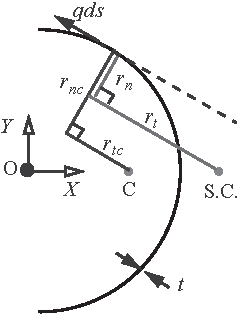
\includegraphics{Figure_4-26.pdf}
\vspace*{-18pt}
\caption{The shear flow located from the centroid and shear center by coordinates tangent and normal to the contour.\label{fig4.26}}
\vspace*{6pt}
\end{wrapfigure}

\noindent respect to the centroid as shown in figure~\ref{fig4.26}. In this example the normal coordinate with respect to the centroid is
\begin{align}\label{ex4.7j}
r_{n}=a\left(1-\frac{4}{\pi} \cos \theta\right),\end{align}
Substitute eq. (\textbf{\ref{ex4.7k}}) for $r_{n}(\theta)$ in eq. (\textbf{i}) followed by substitution eq. (\textbf{\ref{ex4.7f}}) for the shear flow to get
\begin{align}\label{ex4.7k}
M_{z}&=\int_{-\pi/2}^{\pi/2}\left[a\left(1-\frac{4}{\pi} \cos \theta\right)\right]\left[\frac{2 V_{y}}{(a \pi)} \cos \theta\right] a d \theta\nonumber\\[5pt]
&=\frac{2 a}{\pi} V_{y} \int_{-\pi/2}^{\pi/2}\left[\cos \theta-\frac{4}{\pi} \cos ^{2} \theta\right] d \theta
\nonumber\\[2pt]
&=\left.\frac{2 a}{\pi} V_{y}\left[\sin \theta-\frac{4}{\pi}\left(\frac{\theta}{2}+\frac{1}{4} \sin 2 \theta\right)\right]\right|_{-\pi/2} ^{\pi/2}.\end{align}
Evaluating eq. (\textbf{k}) we find
\begin{align}\label{ex4.7l}
M_{z} =\frac{2 a}{\pi} V_{y}\left[1-(-1)-\frac{4}{\pi}\left[\frac{\pi}{4}-\left(-\frac{\pi}{4}\right)+\frac{1}{4}(0-0)\right]\right]
=\frac{2 a}{\pi} V_{y}\left[2-\frac{4}{\pi}\left[\frac{\pi}{2}+\frac{1}{4}(0-0)\right]\right]=\frac{2 a}{\pi} V_{y}[2-2]=0.
\end{align}
The result of the integration given by eq. (\textbf{l}) verifies that the shear flow results in no torque at the shear center.

\subsubsection{Solution to part (d).} The shear stress $\sigma_{z s}$ is the sum of the shear stresses from the transverse shear force ${V}_y$ and from the torque $M_{z}$, and is given by eq.~(\ref{eq4.12}) on page \pageref{eq4.12}. For this example we find
\begin{align}\label{ex4.7m}
\sigma_{z s}=q/t+2\left(M_{z}/J\right) \zeta=2\left(V_{y}/A\right) \cos \theta+2\left(M_{z}/J\right) \zeta \quad-\pi/2 \leq \theta \leq \pi/2 \quad-t/2 \leq \zeta \leq t/2.
\end{align}
From eq.~(\ref{eq4.14}) the torsion constant $J=\left(b t^{3}\right)/3=\left(a \pi t^{3}\right)/3$. The shear stress (\textbf{m}) is a maximum at $\theta = 0$, where the shear flow is maximum. At $\theta = 0$ the maximum shear stress is determined\vspace*{-2pt} from
\begin{align}\label{ex4.7n}
\left.\sigma_{z s}\right|_{\theta=0}=2\left(V_{y}/A\right) \pm\left(M_{z}/J\right) t.
\end{align}\hfill\qed
\end{example*}



\begin{wrapfigure}[6]{r}{116pt}
%\vspace{-19pt}
\vspace*{3pt}
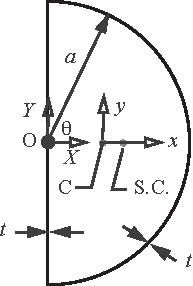
\includegraphics{Figure_4-27.pdf}
\caption{Closed contour.\label{fig4.27}}
\end{wrapfigure}
\vspace*{-2\baselineskip}
\begin{example*}[Shear stress analysis for a closed cross-sectional contour]\label{ex4.8}\setcounter{equation}{0}\def\theequation{\alph{equation}}%
A closed contour in the shape of the letter D is shown in figure~\ref{fig4.27}. The origin of the \textit{X-Y} system is taken at the center of the semicircular branch. The cross section is symmetric about the \textit{X}-axis, so the centroid and shear center lie on the \textit{X}-axis. To locate the shear center we take shear force $V_{x}=0$, and note that the shear force $V_{y} \neq 0$ and torque $M_{z} \neq 0$ act at the shear center.

\begin{enumerate}[b)]
  \item[a)] Locate the centroid,
  \item[b)] determine the shear flow with respect to the centroid,
  \item[c)] locate the shear center,
  \item[d)] establish the shear flow with respect to the shear center, and
  \item[e)] determine the shear stress $\sigma_{z s}$.
\end{enumerate}


\subsubsection{Solution to part (a).} The cross section is composed of two branches. Branch 1 is the semicircular contour, and branch 2 is the vertical web connecting the ends of branch 1. The parametric equations of the contour for each branch are
\begin{align}\label{ex4.8a}
\begin{array}{@{}cc@{}}{\left[X_{1}(\theta), Y_{1}(\theta)\right]=a[\cos (\theta), \sin (\theta)]} & -\pi/2 \leq \theta \leq \pi/2 \\{\left[X_{2}(s), Y_{2}(s)\right]=[0, a-s]} & 0 \leq s \leq 2 a\end{array}.
\end{align}
Note that the contour coordinate $s$ in branch 2 is defined in the negative $y$-direction. We compute the area \textit{A}, the first area moment about the \textit{Y}-axis $Q_{Y}$, and the location of the centroid as follows:
\begin{align}\label{ex4.8b}
A=\int_{-\pi/2}^{\pi/2} t a d \theta+\int_{0}^{2a} t d s=(2+\pi) a t \quad Q_{Y}=\int_{-\pi/2}^{\pi/2} X_{1} t a d \theta+\int_{0}^{2a} X_{2} t d s=2 a^{2} t \quad X_{C}=\frac{Q_{Y}}{A}=\frac{2 a}{2+\pi}.
\end{align}

\subsubsection{Solution part to (b).} The shear flow relative to the centroid is given by eq.~(\ref{eq4.17}) on page~\pageref{eq4.17}. For this example this shear flow function\vspace*{-3pt} is
\begin{align}\label{ex4.8c}
q_{C}(s, z)=\frac{M_{z c}(z)}{2 A_{c}}-F_{y c}(s) V_{y}(z),
\end{align}
The function $F_{y c}(s)$ is given by eq.~(\ref{eq4.19}). For this symmetric section the product area moment $I_{x y}=0$, and from eq.~(\ref{eq4.4}) on page~\pageref{eq4.4} the cross-sectional coefficients $n_{x}=n_{y}=0$ and $k=1$. Also, from eq.~(\ref{eq4.7}) $\bar{y}(s)=y(s)$. The function $F_{y c}(s)$ in eq.~(\ref{eq4.19}) reduces\vspace*{-3pt} to
\begin{align}\label{ex4.8d}
F_{y c}(s)=\frac{1}{I_{x x}}\left[Q_{x}(s)-\frac{1}{\left(2 A_{c}\right)} \oint\! r_{n c}(s) Q_{x}(s) d s\right].
\end{align}
The distribution function given by eq.~(\ref{eq4.23}) in this example is simplified\vspace*{-3pt} to
\begin{align}\label{ex4.8e}
\bar{Q}_{x}=Q_{x}=\int_{0}^{s} y(s) t(s) d s,
\end{align}
and the coordinate normal to the contour $r_{n c}(s)$ in eq. (\textbf{\ref{ex4.8d}}) is given in eq.~(\ref{eq4.10}). The parametric equations of the contour with respect to the centroid\vspace*{-3pt} are
\begin{align}\label{ex4.8f}
\begin{array}{@{}cc@{}}x_{1}(\theta)=X_{1}(\theta)-X_{C}=\displaystyle\frac{-2 a}{2+\pi}+a \cos \theta & y_{1}(\theta)=Y_{1}(\theta) \\[10pt]
x_{2}(s)=X_{2}(s)-X_{C}=\displaystyle\frac{-2 a}{2+\pi} \quad y_{2}(s)=Y_{2}(s)\end{array}.
\end{align}
The second area moment of the cross section about the $x$-axis through the centroid is
\begin{align}\label{ex4.8g}
I_{x x}=\int_{-\pi/2}^{\pi/2} y_{1}^{2} t a d \theta+\int_{0}^{2 a} y_{2}^{2} t d s=\left(\frac{4+3 \pi}{6}\right) a^{3} t=2.23746 a^{3} t.
\end{align}

\removelastskip

The distribution function about the $x$-axis beginning at the contour origin at $\theta=-\pi/2$ and going counterclockwise around the contour are determined for each branch from eq. (\textbf{\ref{ex4.8e}}) as
\begin{align}\label{ex4.8h}
Q_{x 1}(\theta)&=\int_{-\pi/2}^{\theta} y_{1} t a d \theta=-a^{2} t \cos \theta \quad-\pi/2 \leq \theta \leq \pi/2, \text{and}\\
Q_{x 2}(s)&=Q_{x 1}(\pi/2)+\int_{0}^{s} y_{2} t d s=a t s-t\left(\frac{s^{2}}{2}\right) \quad 0 \leq s \leq 2 a.\label{ex4.8i}
\end{align}
\vspace*{4pt}
\clearpage

\noindent Note that $Q_{x 2}(2 a)=0$, since this represents the first area moment of the entire cross section about the centroidal $x$-axis. From eq.~(\ref{eq4.10}) the coordinates normal to the contour for each branch are
\begin{align}\label{ex4.8j}
r_{n c 1}=x_{1}\left(\frac{d y_{1}}{a d \theta}\right)-y_{1}\left(\frac{d x_{1}}{a d \theta}\right)=a\left(1-\frac{2}{2+\pi} \cos \theta\right) \quad r_{n c 2}=x_{2}\left(\frac{d y_{2}}{d s}\right)-y_{2}\left(\frac{d x_{2}}{d s}\right)=\frac{2 a}{2+\pi}.
\end{align}
The area enclosed by the closed contour $A_{c}$ is given by eq.~(\ref{eq4.18}), and we get the expected result as shown below.
\begin{align}\label{ex4.8k}
A_{c}=\int_{-\pi/2}^{\pi/2} r_{n c 1} a d \theta+\int_{0}^{2a} r_{n c 2} d s=\pi a^{2}/2.
\end{align}
Let the term containing the integral over the entire contour in eq. (\textbf{d}) be denoted by $F_{y c 0}$. We compute $F_{y c 0}$ for this cross section as
\begin{align}\label{ex4.8l}
F_{y c 0}=\frac{1}{\left(2 A_{c}\right)} \oint\! r_{n c}(s) Q_{x}(s) d s=\frac{1}{2 A_{c}}\left(\int_{-\pi/2}^{\pi/2} r_{n c 1} Q_{x 1} a d \theta+\int_{0}^{2a} r_{n c 2} Q_{x 2} d s\right)=-\frac{8+3 \pi}{3 \pi(2+\pi)}(a^{2} t).
\end{align}
We now compute the shear flow distribution functions for each branch by substituting results from eqs. (\textbf{\ref{ex4.8h}}), (\textbf{\ref{ex4.8i}}), and (\textbf{\ref{ex4.8l}}) into eq. (\textbf{\ref{ex4.8d}}). The results are
\begin{align}\label{ex4.8m}
F_{y c 1}&=\frac{\left(Q_{x 1}-F_{y c 0}\right)}{I_{x x}}=\frac{1}{a}(0.16071-0.446935 \cos \theta), \text{and}
\\
F_{y c 2}&=\frac{(Q_{x 2}-F_{y c 0})}{I_{x x}}=\frac{1}{a}(0.16071+0.446935(s/a)-0.223467(s/ a)^{2}).\label{ex4.8n}
\end{align}
The shear flows with respect to the centroid in branch 1 and branch 2 are
\begin{align}\label{ex4.8o}
q_{C 1}(s, z)=\frac{M_{z c}(z)}{2 A_{c}}-F_{y c 1}(\theta) V_{y}(z) \quad q_{C 2}(s, z)=\frac{M_{z c}(z)}{2 A_{c}}-F_{y c 2}(\theta) V_{y}(z).
\end{align}

\vspace*{-10pt}

\subsubsection{Solution to part (c).} The equation for the location of the shear center relative to the centroid is given in eq.~(\ref{eq4.23}). The shear modulus of the material is denoted by \textit{G} in eq.~(\ref{eq4.23}), and we assume it is uniform around the contour in this example. Then the shear center relative to the centroid is
\begin{align}\label{ex4.8p}
x_{s c}=\frac{2 A_{c}}{\oint\! d s}\left[\int_{-\pi/2}^{\pi/2} F_{y c 1} a d \theta+\int_{0}^{2a} F_{y c 2} d s\right], \text{where}\ \oint\! d s=\int_{-\pi/2}^{\pi/2} a d \theta+\int_{0}^{2 a} d s=(2+\pi) a,
\end{align}
Performing the integrals for $x_{s c}$ in eq. (\textbf{\ref{ex4.8p}}) we get
\begin{align}\label{ex4.8q}
x_{s c}=\frac{\pi a^{2}/2}{(2+\pi) a}\left[\frac{16-2 \pi}{4 \pi+3 \pi^{2}}\right]=\frac{(16-2 \pi)}{(2+\pi)(4+3 \pi)} a=0.140773 a.
\end{align}
The location of the shear center relative to point O is $X_{S C}=X_{C}+x_{s c}=0.529757 a$.

\subsubsection{Solution to part (d).} The shear flow relative to the shear center is given by eq.~(\ref{eq4.25}), which in this example is
\begin{align}\label{ex4.8r}
q(s, z)=\frac{M_{z}(z)}{2 A_{c}}-F_{y}(s) V_{y}(z),
\end{align}

\pagebreak

\noindent where the shear flow distribution function relative to the shear center is given by eq.~(\ref{eq4.26}). The results for the shear flow distribution functions relative to the shear center for each branch are as follows:
\begin{gather}\label{ex4.8s}
F_{y 1}=-\left(\frac{x_{s c}}{2 A_{c}}\right)+F_{y c 1}=\frac{1}{a}(0.1159-0.445635 \cos \theta), \text{and}
\\[6pt]
F_{y 2}=-\left(\frac{x_{s c}}{2 A_{c}}\right)+F_{y c 2}=\frac{1}{a}\left[0.1159+0.446935\left(\frac{s}{a}\right)-0.223467\left(\frac{s}{a}\right)^{2}\right].\label{ex4.8t}
\end{gather}
Finally, from eq. (\textbf{r}) the shear flows in each branch are given by
\begin{gather}
q_{1}=\frac{M_{z}}{2 A_{c}}-F_{y 1} V_{y}=\frac{M_{z}}{\pi a^{2}}-\frac{1}{a}(0.1159-0.445635 \cos \theta) V_{y}, \text{and}
\label{ex4.8u}\\[6pt]
q_{2}=\frac{M_{z}}{2 A_{c}}-F_{y 2} V_{y}=\frac{M_{z}}{\pi a^{2}}-\frac{1}{a}\left[0.1159+0.446935\left(\frac{s}{a}\right)-0.223467\left(\frac{s}{a}\right)^{2}\right].\label{ex4.8v}
\end{gather}

A check on the shear flows is to compute the resultant for $F_{y}$ and the resultant moment about the shear center $C_{z}$. Resolving the shear flows in the positive $y$-direction in each branch we compute the integrals
\[
F_{y}=\int_{-\pi/2}^{\pi/2} q_{1} \cos \theta a d \theta-\int_{0}^{2a} q_{2} d s=V_{y}.
\]
Thus, the resultant $F_{y}$ is equal to the shear force. Note that  $q_2$  is positive in the negative $y$-direction. To compute the moment $C_{z}$ we need the normal coordinate to the contour with respect to the shear center. From eq.~(\ref{eq4.11}) on page~\pageref{eq4.11} the normal coordinates for each branch are determined by
\begin{align}\label{ex4.8w}
r_{n 1}=r_{n c 1}-x_{s c}\left(\frac{d y_{1}}{a d \theta}\right)=a(1-0.529757 \cos \theta) \quad r_{n 2}=r_{n c 2}-x_{s c}\left(\frac{d y_{2}}{d s}\right)=0.529757 a.
\end{align}
The resultant moment is
\begin{align}\label{ex4.8x}
C_{z}=\int_{-\pi/2}^{\pi/2} r_{n 1} q_{1} a d \theta+\int_{0}^{2a} r_{n 2} q_{2} d s=M_{z}.
\end{align}
The moment of the shear flows about the shear center equal the torque $M_{z}$. The shear flows in eqs. (\textbf{\ref{ex4.8u}}) and (\textbf{\ref{ex4.8v}}) are statically equivalent to the shear force $V_{y}$ and the torque $M_{z}$ resolved at the shear center.

\subsubsection{Solution to part (e).} The shear flows are plotted normal to the contour in figure~\ref{fig4.28}. The shear flow from the torque is spatially uniform and equal to $M_{z} /\left(2 A_{c}\right)$. The shear stress is equal to the shear flow divided by the thickness of the branch. From figure~\ref{fig4.28} it is apparent that the maximum magnitude of the shear stress occurs either at $\theta=0$ in the semicircular contour or at $s=a$ in the vertical contour. These shear stress components are
\begin{align}\sigma_{z s 1}(0)=\frac{M_{z}}{\pi a^{2} t}+\frac{0.3297 V_{y}}{a t} \quad \sigma_{z s 2}(a)=\frac{M_{z}}{\pi a^{2} t}-\frac{0.3394 V_{y}}{a t}.
\end{align}\hfill\qed
\end{example*}

\pagebreak

{\def\thefigure{4.28}
\begin{figure}
\centering{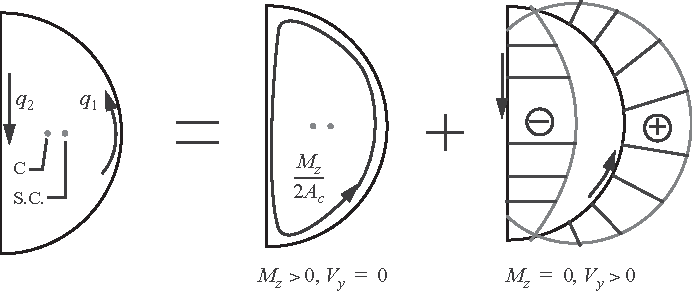
\includegraphics{Figure_4-28.pdf}}
\caption{Shear flow distribution along the contour of the closed section shown in figure \ref{fig4.27}. The shear flow is the sum of a spatially uniform flow due to the torque plus a nonuniform flow due to the shear\break force.\label{fig4.28}}
\end{figure}}

\begin{example}[Torsional response of an open section and an equivalent closed section]\label{ex4.9}\setcounter{equation}{0}\def\theequation{\alph{equation}}%
A thin-walled circular tube with contour radius $a$ and wall thickness $t$ is subject to a torque $M_{z}$. The wall of a second identical tube is cut parallel to its longitudinal axis along its entire length to make the cross section of this second tube an open circular arc. See figure~\ref{fig4.29}. Assume the saw kerf is very small. Compare the unit twist and maximum shear stress in the closed section to the open section.

{\def\thefigure{4.29}
\processfigure[H]{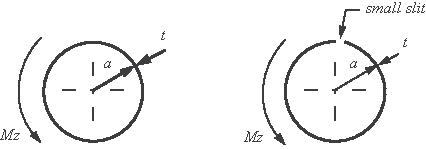
\includegraphics{Figure_4-29.pdf}
}{\caption{Closed and open thin-walled
circular sections.\label{fig4.29}}}}


\noindent\textbf{Solution.}\enspace
For the closed section the shear flow $q=\frac{M_{z}}{2\left(\pi a^{2}\right)}$ as shown in figure~\ref{fig4.28}, and the torsion constant $J=2 \pi a^{3} t$ from eq.~(\ref{eq3.128}) on page~\pageref{eq3.128}. Hence the maximum shear stress and unit twist are
\begin{align}\label{ex4.9a}
\left(\sigma_{z s}\right)_{\textit{closed }}=\frac{M_{z}}{2 \pi a^{2} t} \quad\left(\frac{d \theta_{z}}{d z}\right)_{\textit{closed }}=\frac{M_{z}}{G J}=\frac{M_{z}}{G\left(2 \pi a^{3} t\right)}.
\end{align}

\removelastskip

For the open section the developed length $b$ of the contour is essentially $2 \pi a$, since the saw kerf is assumed to be very small. By the membrane analogy discussed in article \ref{sec3.9.1} on page~\pageref{sec3.9.1}, the torsional response is the same as the thin-walled rectangular section of length $b$ and thickness $t$. The maximum shear stress is given by eq.~(\ref{eq3.129}) on page \pageref{eq3.129}, and the torsion constant is given in eq.~(\ref{eq3.128}). For $b=2 \pi a$, we have
\begin{align}\label{ex4.9b}
\left(\sigma_{z s}\right)_{\textit{open}}=\frac{3 M_{z}}{2 \pi a t^{2}} \quad\left(\frac{d \theta_{z}}{d z}\right)_{\textit{open }}=\frac{M_{z}}{G\left(\frac{1}{3} 2 \pi a t^{3}\right)}.
\end{align}

Forming the ratio of the maximum shear stress of the open section to the closed section we find
\begin{align}\label{ex4.9c}
\frac{(\sigma_{z s})_{\textit{open }}}{(\sigma_{z s})_{\textit{closed }}}=\frac{3 M_{z}}{2 \pi a t^{2}} \cdot \frac{2 \pi a^{2} t}{M_{z}}=3 \frac{a}{t} \gg 1.
\end{align}
Likewise, the ratio of the unit twists are
\begin{align}\label{ex4.9d}
\frac{(d \theta_{z}/d z)_{\textit{open }}}{(d \theta_{z}/d z)_{\textit{closed }}}=\frac{3 M_{z}}{G 2 \pi a t^{3}} \cdot \frac{G 2 \pi a^{3} t}{M_{z}}=3\left(\frac{a}{t}\right)^{2} \gg 1.
\end{align}
Since the ratio of the radius to thickness is greater than ten for a thin-walled section, the above results show that the shear stress (\textbf{\ref{ex4.9c}}) and unit twist (\textbf{\ref{ex4.9d}}) of the open circular section are much larger than for the closed section if both sections are subject to the same torque.

Hence, if a bar is to resist torsional loading, a closed section is preferable to an equivalent open section bar. That is, the unit twist is smaller for the closed section bar (it is stiffer), and the maximum shear stress is smaller, than for the equivalent open section bar subject to the same torque.
\end{example}



\subsection{Resultant of uniform shear flow}\label{sec4.4.1}\setcounter{equation}{51}

\noindent
In torsion problems it is often necessary to find the resultant of a constant shear flow along the contour of a curved branch. This situation is depicted in figure~\ref{fig4.30}, where the curved branch begins at point \textit{A} with coordinates $\left(X_{A}, Y_{A}\right)$ and ends at point \textit{B} with coordinates $\left(X_{B}, Y_{B}\right)$. The resultant of the shear flow is resolved at point A in this figure.

\begin{wrapfigure}[13]{l}{217pt}
\vspace{-30pt}
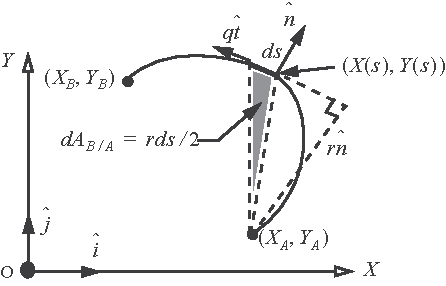
\includegraphics{Figure_4-30.pdf}
\caption{A constant shear flow in a curved
branch.\label{fig4.30}}
\end{wrapfigure}


The sense of the arc-length $s$ and the shear flow $q$ are assumed positive from \textit{A} to \textit{B} along the contour of the branch. The shear flow acts tangent to the contour, and the unit tangent vector to the contour is denoted by $\hat{t}(s)$. The unit tangent vector is given by eq.~(\ref{eq3.4}) on page \pageref{eq3.4}, where we note that $d X/d s=d x/d s$ and $d Y/d s=d y/d s$. The differential force obtained from the shear flow is
\begin{align}\label{eq4.52}
d \harp{F}=q d s \hat{t}=q d s\left[\left(\frac{d X}{d s}\right) \hat{i}+\left(\frac{d Y}{d s}\right) \hat{j}\right]=q[(d X) \hat{i}+(d Y) \hat{j}].
\end{align}
Integrate eq.~(\ref{eq4.52}) from point \textit{A} to point \textit{B} on the contour to get
\begin{align}\label{eq4.53}
\harp{F}=q\left[\int_{A}^{B}\left(d X \hat{i}+d Y_{\hat{j}}\right)\right]=q\left[\left(X_{B}-X_{A}\right) \hat{i}+\left(Y_{B}-Y_{A}\right) \hat{j}\right]=\left(q L_{B/A}\right) \hat{u}_{B/A},
\end{align}
where the length of the chord connecting the ends of contour is denoted by $L_{B/A}$. The length of the chord and the unit vector $\hat{u}_{B/A}$ are given by
\begin{align}\label{eq4.54}
L_{B/A}=\sqrt{\left(X_{B}-X_{A}\right)^{2}+\left(Y_{B}-Y_{A}\right)^{2}} \quad \hat{u}_{B/ A}=\frac{\left(X_{B}-X_{A}\right)}{L_{B/A}} \hat{i}+\frac{\left(Y_{B}-Y_{A}\right)}{L_{B/A}} \hat{j}.
\end{align}
The differential torque about point \textit{A} is
\begin{align}\label{eq4.55}
d \harp{M}_{A}=r(s) \hat{n}(s) \times q d s \hat{t}=q r(s) d s \hat{k},
\end{align}
\vspace*{5pt}
\clearpage

\noindent where the position vector from point \textit{A} to the line of action of the shear flow is $r(s) \hat{n}(s)$, and $\hat{n}(s)$ is the unit vector normal to the contour at $s$. The product of $r$ times \textit{ds} is twice the enclosed area of the triangle with base \textit{ds} and height $r$. As shown in figure~\ref{fig4.30} $r(s) d s=2 d A_{B/A}$. Integrate eq.~(\ref{eq4.55}) from point \textit{A} to point \textit{B} to get
\begin{align}\label{eq4.56}
\harp{M}_{A}=q \int_{A}^{B} r(s) d s \hat{k}=q \int_{A}^{B} 2 d A_{B/A} \hat{k}=2 q A_{B/A} \hat{k}.
\end{align}
The area between the contour and the chord is denoted by $A_{B/A}$. The force and torque resolved at point \textit{A} is shown in figure~\ref{fig4.31}(a). The force and torque at point \textit{A} are statically equivalent to the force acting along a line of action that is parallel to the chord at a perpendicular distance $e$ from the chord. The distance is determined from $M_{A}=e F=e q L_{A/B}$. Solve for $e$ and substitute $2 q A_{B/A}$ for the torque to get
{\def\thefigure{4.31}
\processfigure[H]{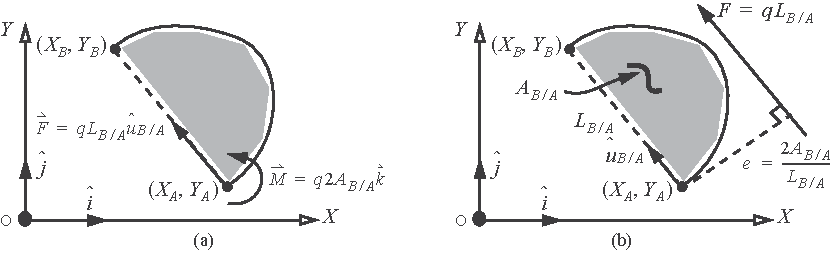
\includegraphics{Figure_4-31.pdf}
}{\caption{(a) The force and torque due to a constant shear flow resolved at point $A$. (b) The resultant of a constant shear flow is a force parallel to the chord at distance $e$ from it.\label{fig4.31}}\vspace*{-10pt}}}

\vspace*{-2\baselineskip}
\begin{align}\label{eq4.57}
e=\frac{M_{A}}{q L_{B/A}}=\frac{2 q A_{B/A}}{q L_{B/A}},\ \text{or}\ e=\frac{2 A_{B/A}}{L_{B/A}}.
\end{align}


\noindent The resultant of a constant shear flow is shown in figure~\ref{fig4.31}(b).


\begin{wrapfigure}[10]{r}{128pt}
\vspace{-32pt}
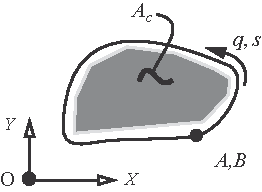
\includegraphics{Figure_4-32.pdf}
\caption{Constant shear flow on a closed contour of arbitrary shape.\label{fig4.32}}
\end{wrapfigure}

Now consider a continuous contour that does not intersect itself except that point \textit{B} coincides with point \textit{A} as shown in figure~\ref{fig4.32}. Since $L_{B/A}=0$ in eq.~(\ref{eq4.53}) the force $\harp{F}=0$. For a closed contour let $A_{B/A}=A_{c}$ and $M_{A}=M_{z}$ in eq.~(\ref{eq4.56}). For a single-cell cross section subject to a torque $M_{z}$ and no shear forces (pure torsion), the shear flow is given by\vspace*{3pt}
\begin{align}\label{eq4.58}
q=\frac{M_{z}}{2 A_{c}}.
\end{align}

\removelastskip

\noindent Equation (\ref{eq4.58}) is called \textbf{Bredt's formula}. (Also see eq.~(\ref{eq3.165}) on page \pageref{eq3.165},)

A constant shear flow in a closed contour is statically equivalent to a torque, and this torque is the same for any point in the plane about which moments are computed. The fact that the torque is a ``free vector'' is depicted in figure~\ref{fig4.33}, in which it is shown that some of the enclosed area used in Bredt's formula can add as a negative quantity if the torque produced by the constant shear flow is clockwise over a segment of the branch. About point O in this figure, the torque produced by the shear flow from point \textit{B} to \textit{A} in the right half of the contour is counterclockwise, and the torque produced by the shear flow from \textit{A} to \textit{B} in the left half is clockwise. Hence, the total torque is the sum of these two torques with due respect to the sign. This summation shows that the total torque is proportional to the area enclosed by the contour.

\pagebreak

{\def\thefigure{4.33}
\processfigure[H]{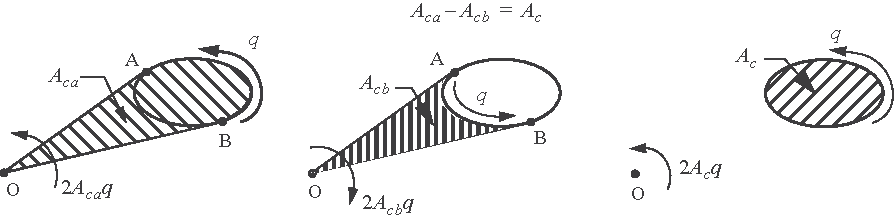
\includegraphics{Figure_4-33.pdf}
}{\caption{The torque about an arbitrary point O of a constant shear flow in a closed contour is twice the enclosed area of the circuit times the shear flow.\label{fig4.33}}}}



\begin{wrapfigure}[12]{L}{172pt}
%\vspace{-19pt}
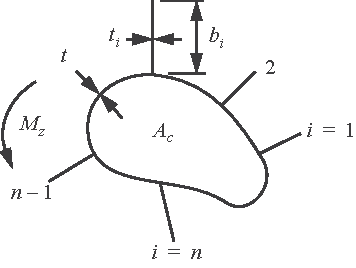
\includegraphics{Figure_4-34.pdf}
\caption{Torsion of a hybrid section.\label{fig4.34}}
\end{wrapfigure}

\subsection{Torsion of a hybrid section}\label{sec4.4.2}

Consider a hybrid section composed of a single closed cell and open branches, or fins, as shown in figure~\ref{fig4.34}. The total torque carried by the section is the sum of the torques carried by the closed cell and open branches. For $n$ open branches, we have
\begin{align}\label{eq4.59}
M_{z}=\left(M_{z}\right)_{\textit{closed}}+\sum_{i=1}^{n}\left(M_{z}\right)_{i},
\end{align}
where
\begin{align}\label{eq4.60}
\left(M_{z}\right)_{\textit{closed }}=(G J)_{\textit{closed }}\left(\frac{d \phi_{z}}{d z}\right)\ \text{and}\ \left(M_{z}\right)_{i}=(G J)_{i}\left(\frac{d \phi_{z}}{d z}\right).
\end{align}
\noindent The torsional stiffness for the closed cell is
\begin{align}\label{eq4.61}
(G J)_{\textit{closed }}=\frac{4 A_{c}^{2}}{\oint\! \frac{d s}{G t}},
\end{align}
and for each open branch the torsional stiffness is
\begin{align}\label{eq4.62}
(G J)_{i}=G_{i}\left(\frac{1}{3} b_{i} t_{i}^{3}\right).
\end{align}
\vspace*{-\baselineskip}

\noindent Combining eqs. (\ref{eq4.59}) and (\ref{eq4.60}), we have
\begin{align}\label{eq4.63}
M_{z}=\left[(G J)_{\textit{closed }}+\sum_{i=1}^{n}(G J)_{i}\right\rfloor \frac{d \phi_{z}}{d z}.
\end{align}
Comparing eq.~(\ref{eq4.63}) to the standard torsional formula $M_{z}=(G J)_{\textit{eff}}\left(\frac{d \phi_{z}}{d z}\right)$, the effective torsional stiffness for the entire section is\vspace*{-5pt}
\begin{align}\label{eq4.64}
(G J)_{\textit{eff}}=(G J)_{\textit{closed}}+\sum_{i=1}^{n}(G J)_{i}.
\end{align}
where the closed and open parts of the torsional stiffness are given by eqs. (\ref{eq4.61}) and (\ref{eq4.62}).

\vfill\pagebreak

The shear stress in the closed cell is $\left(\sigma_{z s}\right)_{\textit{closed}}=\left(M_{z}\right)_{\textit{closed}} /\left(2 A_{c} t\right)$, where the portion of the torque carried by the closed cell is $\left(M_{z}\right)_{\textit{closed }}=(G J)_{\textit{closed }}\left(d \phi_{z}/d z\right)$. The unit twist is given by $\left(d \phi_{z}/d z\right)=M_{z} /(G J)_{\textit{eff}}$. Combining these results, the shear stress in the closed cell is
\begin{align}\label{eq4.65}
\left(\sigma_{z s}\right)_{\textit{closed}}=\frac{(G J)_{\textit{closed}}}{(G J)_{\textit{eff}}} \cdot \frac{M_{z}}{2 A_{c} t}\end{align}
The shear stress in open branches is given by
\begin{align}\label{eq4.66}
\left(\left.\sigma_{z s}\right|_{\max }\right)_{i}=\frac{3 M_{z i}}{b_{i} t_{i}^{2}},
\end{align}
which was derived as eq.~(\ref{eq3.132}) on page \pageref{eq3.132}. Substitute the second equation in (\ref{eq4.60}) for the torque carried by the branch, and then substitute eq.~(\ref{eq4.62}) for the torsional stiffness of the branch, to write the shear stress as
\begin{align}\label{eq4.67}
\left(\sigma_{z s}\right)_{i}=\frac{3\left(M_{z}\right)_{i}}{b_{i} t_{i}^{2}}=\frac{3}{b_{i} t_{i}^{2}} \cdot\left(G_{i} \frac{1}{3} b_{i} t_{i}^{3}\right) \frac{d \phi_{z}}{d z}.
\end{align}
Substitute $\frac{d \phi_{z}}{d z}=\frac{M_{z}}{(G J)_{\textit{eff}}}$ for the unit twist in eq.~(\ref{eq4.67}) to get
\begin{align}\label{eq4.68}
\left(\sigma_{z s}\right)_{i}=\frac{G_{i} t_{i}}{(G J)_{\textit{eff}}} M_{z}.
\end{align}
If the shear modulus is the same in all branches, then eqs. (\ref{eq4.65}) and (\ref{eq4.68}) reduce to
\begin{align}\label{eq4.69}
\left(\sigma_{z s}\right)_{\textit{closed}}=\frac{J_{\textit{closed}}}{J_{\textit{eff}}} \cdot \frac{M_{z}}{2 A_{c} t} \quad\left(\sigma_{z s}\right)_{i}=\frac{t_{i} M_{z}}{J_{\textit{eff}}},
\end{align}
where $J_{\textit{eff}}=J_{\textit{closed }}+\displaystyle\sum\limits_{i=1}^{n} J_{i}$.




\begin{example*}[Torsion of a closed cross section composed of two cells]\label{ex4.10}In multicell cross sections subject to pure torsion the shear flow is constant in each branch. In general the shear flows are different from branch to branch. Consider a cross section consisting of two cells with a horizontal axis of symmetry shown in figure~\ref{fig4.35}. It is subject to a torque ${M}_z$. Cell 1 is enclosed by a semicircular exterior web of radius $a$, and a vertical web of length 2\textit{a}, which is common with cell 2. Cell 2 is enclosed by an isosceles triangle with equal exterior webs of length $c$ and the common web of length $2a$. Take $a = 5$ in., $b = 12$ in., and $c = 13$ in. The thickness of the exterior webs $t = 0.040$ in., and the thickness of the common web is $t/2$. The contour is composed of four branches. Branch 1 is the semicircular web with the contour coordinate denoted by $s_1$, branch 2 is the upper exterior straight web of cell 2 with contour coordinate $s_2$, branch 3 is the lower exterior straight web of cell 2 with contour coordinate $s_3$, and branch 4 is the vertical common web between cells with the contour coordinate denoted by $s_{\textrm{1-2}}$.The Cartesian coordinate system \textit{X-Y} has its origin at point O, the center of the semicircular web. The \textit{X}-axis is the axis of symmetry.

\pagebreak

{\def\thefigure{4.35}
\processfigure[H]{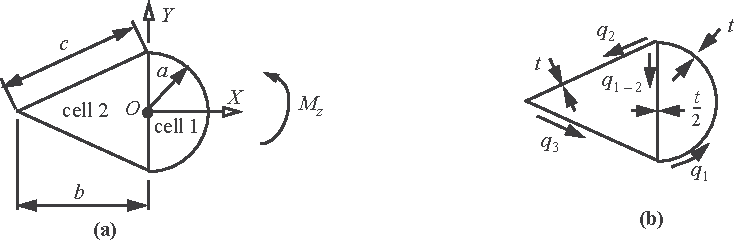
\includegraphics{Figure_4-35.pdf}
}{\caption{(a) Cross section composed of two cells and subject to pure torsion. (b) Shear flows and web thicknesses.\label{fig4.35}}}}



A free body diagram of the junction between branches 1, 2, and 1-2 is shown in figure~\ref{fig4.36}. The sum of forces in the axial direction is $q_{\textrm{1-2}} \Delta z+q_{2} \Delta z-q_{1} \Delta z=0$, Hence, axial equilibrium per unit $z$-length determines the shear flow in the common web as
\begin{align}\label{ex4.10a}
q_{\textrm{1-2}}=q_{1}-q_{2}.\tag{a}
\end{align}

\vspace*{-3\baselineskip}
{\def\thefigure{4.36}
\processfigure[H]{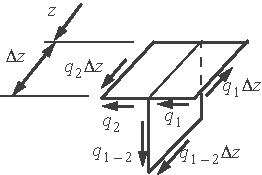
\includegraphics{Figure_4-36.pdf}
}{\caption{Free body diagram of the junction between
branches 1, 2,\break and 1-2.\label{fig4.36}}}}
\vspace*{-1\baselineskip}

\noindent A simple rule to determine the axial equilibrium of the junction is to observe that the shear flow into the junction must equal the shear flow out of the junction. At the junction of branches 2 and 3 this rule results in $q_{3}=q_{2}$. At the junction of branches 3, 1-2, and 1 the rule gives $q_{\textrm{1-2}}+q_{3}-q_{1}=0$, but $q_{3}=q_{2}$, which leads us to the same relation given by eq. (\textbf{\ref{ex4.10a}}). We started with four unknown shear flows $q_1$, $q_2$, $q_3$, and $q_{\textrm{1-2}}$. Axial equilibrium at the three junctions results in two relations between the four shear flows. Two shear flows remain unknown, say $q_1$ and  $q_2$, at this point in the analysis.

The remaining equation of static equivalence is to equate the torque due to the shear flows to ${M}_z$. The constant shear flows in each branch are shown in figure~\ref{fig4.37}(a), and the resultants of these shear flows are determined by the analysis presented in article \ref{sec4.4.1}. As shown in figure~\ref{fig4.37}(b) the resultant of the shear flow $q_{1}$ in branch 1 is a vertical upward force of magnitude $2 a q_{1}$, the resultant of the shear flow $q_{2}$ in branches 2 and 3 is a vertical downward force of magnitude $2 a q_{2}$, and the resultant of the shear flow in the common branch is a downward force of magnitude $2 a\left(q_{1}-q_{2}\right)$. The locations of the lines of action of the force resultants with respect to the common branch are also shown in figure~\ref{fig4.37}(b). The vertical force \textit{F} shown in figure~\ref{fig4.37}(c) is determined from the branch forces by equilibrium. The result is
\begin{align}\label{ex4.10b}
F=2 a q_{1}-2 a q_{2}-2 a\left(q_{1}-q_{2}\right)=0.\tag{b}
\end{align}
Take the moment of the branch forces in figure~\ref{fig4.37}(b) about the common web to determine the torque ${M}_z$ shown in figure~\ref{fig4.37}(c). The result for static equivalence of the torque is\pagebreak
\begin{align}\label{eq4.70}
\left(\frac{2 A_{c 1}}{2 a}\right) 2 a q_{1}+\left(\frac{2 A_{c 2}}{2 a}\right) 2 a q_{2}=M_{z},\ \text{or}\nonumber\\
2 A_{c 1} q_{1}+2 A_{c 2} q_{2}=M_{z}.
\end{align}
Equation (\ref{eq4.70}) is the extension of Bredt's formula in eq.~(\ref{eq4.58}) to two cells.

{\def\thefigure{4.37}
\processfigure[H]{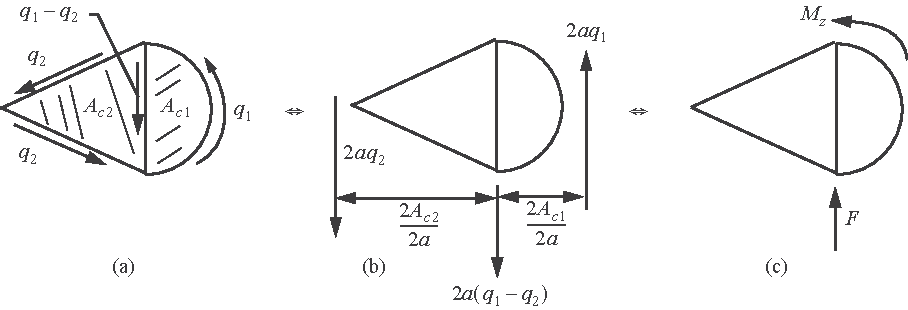
\includegraphics{Figure_4-37.pdf}
}{\caption{(a) Shear flows. (b) Statically equivalent branch forces. (c) Cross section resultant.\label{fig4.37}}}}

\vspace*{-\baselineskip}
We have used all the conditions of static equivalence, but the two shear flows $q_1$ and  $q_2$  remain unknown. An additional equation relating the shear flows is based on the assumed rigidity of the cross section in its own plane. In torsion, this rigid cross section condition implies the unit twist of each cell is the same. The unit twist for a single cell is given by eq.~(\ref{eq4.20}) on page \pageref{eq4.20}. Since the shear modulus is the same for all branches in the cross section eq.~(\ref{eq4.20}) reduces to\vspace*{-5pt}
\begin{align}\label{eq4.71}
\frac{d \phi_{z}}{d z}=\frac{1}{2 A_{c} G} \oint\! \frac{q}{t} ds.
\end{align}
This unit twist formula was derived on the basis that a counterclockwise shear flow tends to produce a counter-clockwise unit twist. Apply this equation to cell 1 to get
\begin{align}\label{ex4.10c}
\left(\frac{d \phi_{z}}{d z}\right)_{1}=\frac{1}{2 A_{c 1} G}\left[\left(\frac{\pi a}{t}\right) q_{1}+\left(\frac{2 a}{t/ 2}\right)\left(q_{1}-q_{2}\right)\right].\tag{c}
\end{align}
For cell 2, the unit twist is\vspace*{-5pt}
\begin{align}\label{ex4.10d}
\left(\frac{d \phi_{z}}{d z}\right)_{2}=\frac{1}{2 A_{c 2} G}\left[\left(\frac{2 c}{t}\right) q_{2}-\left(\frac{2 a}{t/ 2}\right)\left(q_{1}-q_{2}\right)\right].\tag{d}
\end{align}
Note that the contribution of the common branch shear flow is negative in the unit twist formula for cell 2. Relative to an observer in cell 2, a positive value for the shear flow $q_{\textrm{1-2}}$ tends to produce a clockwise unit twist, and hence is negative by the convention that counterclockwise is positive. Since the unit twist of each cell is the same, we equate eqs. (\textbf{\ref{ex4.10c}}) and (\textbf{\ref{ex4.10d}}) to get
\begin{align}\label{ex4.10e}
\frac{1}{A_{c 1}}\left[\left(\frac{2 a}{t}\right) q_{1}+\left(\frac{2 a}{t/ 2}\right)\left(q_{1}-q_{2}\right)\right]=\frac{1}{A_{c 2}}\left[\left(\frac{2 c}{t}\right) q_{2}-\left(\frac{2 a}{t/ 2}\right)\left(q_{1}-q_{2}\right)\right].\tag{e}
\end{align}
After some algebraic manipulations eq. (\textbf{\ref{ex4.10e}}) is written in the form\pagebreak
\begin{align}\label{ex4.10f}
\left[\frac{4 a+a \pi}{A_{c 1} t}+\frac{4 a}{A_{c 2} t}\right] q_{1}-\left[\frac{4 a}{A c_{1} t}+\frac{4 a+2 c}{A_{c 2} t}\right] q_{2}=0.\tag{f}
\end{align}
The enclosed areas of each cell are $A_{c 1}=\pi a^{2}$. and $A_{c 2}=\frac{1}{2} b 2 a=b a$. Numerical evaluations of eqs. (\ref{eq4.70}) and (\textbf{\ref{ex4.10f}}) are
\begin{align}\label{ex4.10g}
\begin{gathered}(50 \pi\,\textrm{in}.^{2}) q_{1}+(120\,\textrm{in}.^{2}) q_{2}=M_{z} \\
(19.6995\,\textrm{in}.^{-2}) q_{1}-(25.5329\,\textrm{in}.^{-2}) q_{2}=0\tag{g}\end{gathered}.
\end{align}
The solutions of the two equations in (\textbf{\ref{ex4.10g}}) for the shear flows are
\begin{align}\label{ex4.10h}
q_{1}=(4.00538 \times 10^{-3}\,\textrm{in}.^{-2}) M_{z} \quad q_{2}=(3.00903 \times 10^{-3}\,\textrm{in}.^{-2}) M_{z} \quad q_{\textrm{1-2}}=(0.915085 \times 10^{-3}\,\textrm{in}.^{-2}) M_{z}.\tag{h}
\end{align}
The shear stresses in each branch are obtained from $\left(\sigma_{z s}\right)_{1}=q_{1}/t$, $\left(\sigma_{z s}\right)_{2}=q_{2}/t$, and $\left(\sigma_{z s}\right)_{\textrm{1-2}}=q_{\textrm{1-2}} /(t/2)$. The results are
\begin{align}\label{ex4.10i}
(\sigma_{z s})_{1}=(0.100135\,\textrm{in}.^{-3}) M_{z} \quad(\sigma_{z s})_{2}=(0.0772575\,\textrm{in}.^{-3}) M_{z} \quad(\sigma_{z s})_{\textrm{1-2}}=(0.0457542\,\textrm{in}.^{-3}) M_{z}.\tag{i}
\end{align}
The twist per unit length for the entire cross section is obtained from either eq. (\textbf{\ref{ex4.10c}}) or eq. (\textbf{\ref{ex4.10d}}). For the shear flows given in eq. (\textbf{\ref{ex4.10h}}) the evaluation of unit twist is
\begin{align}\label{ex4.10j}
\frac{d \phi_{z}}{d z}=\left(\frac{d \phi_{z}}{d z}\right)_{1}=\left(\frac{d \phi_{z}}{d z}\right)_{2}=(0.0129263\,\textrm{in}.^{-4})(M_{z}/G).\tag{j}
\end{align}
Finally, we compute the torsion constant \textit{J} by the following relation
\begin{align}\label{ex4.10k}
J=\frac{M_{z}}{G\left(\frac{d \phi_{z}}{d z}\right)}=77.3619\,\textrm{in}.^{4}\tag{k}\\[-30pt]
\ \nonumber
\end{align}\hfill\qed
\end{example*}

\vspace*{-\baselineskip}
\begin{example}[Torsion of a closed section with three cells; circuit shear flow]\label{ex4.11}\setcounter{equation}{0}\def\theequation{\alph{equation}}Consider the cross section composed of three cells shown in figure~\ref{fig4.38}(a). All branches have the same thickness $t$ and shear modulus \textit{G}. It is convenient to define \textbf{circuit shear flows} in each cell. Circuit shear flows are assumed to be positive counterclockwise in each cell and are equal to the actual shear flows in the exterior branches of the cell, if there are any exterior branches. However, the shear flow in a common branch between cells is the difference between the circuit shear flows sharing the common branch. At the junction of the three branches shown in figure~\ref{fig4.38}(b) the shear flow into the junction is $q_{1}-q_{2}$, and this equals the shear flow out of the junction, which is $\left(q_{1}-q_{3}\right)+\left(q_{3}-q_{2}\right)$. The method of defining circuit shear flows automatically satisfies axial equilibrium at the junction.

For an applied torque $M_{z}$, determine
\begin{itemize}
  \item shear flows $q_1$,  $q_2$, and $q_3$,
  \item the torsion constant \textit{J}, and
  \item magnitude of the torque at the initiation of yielding.
\end{itemize}


{\def\thefigure{4.38}
\processfigure[H]{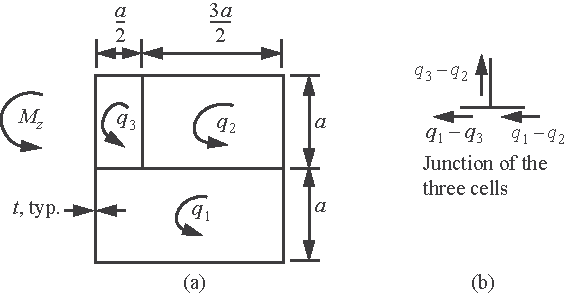
\includegraphics{Figure_4-38.pdf}
}{\caption{(a)
Circuit shear flows in the three-cell cross section.\break (b) Circuit shear flows at the\break junction of the
three cells.\label{fig4.38}}}}


\noindent\textbf{Solution.}\enspace Bredt's formula for the section composed of two cells in eq.~(\ref{eq4.70}) is extended to three cells in this example to get
\begin{align}\label{ex4.11a}
2 A_{c 1} q_{1}+2 A_{c 2} q_{2}+2 A_{3} q_{3}=M_{z}.
\end{align}
The areas enclosed by cells are
\begin{align}\label{ex4.11b}
A_{c 1}=2 a^{2} \quad A_{c 2}=3 a^{2}/2 \quad A_{c 3}=a^{2}/2.
\end{align}
From eq.~(\ref{eq4.71}) the twist per unit length for this example reduces to
\begin{align}\label{ex4.11c}
\frac{d \phi_{z}}{d z}=\frac{1}{2 A_{c} G t} \oint\! q d s=\frac{1}{2 A_{c} G t} \sum \Delta s q.
\end{align}
We apply eq.~(\textbf{\ref{ex4.11c}}) to each cell and note that a shear flow is positive counterclockwise consistent with a positive counterclockwise unit twist. The results for each cell are as follows.
\begin{align}
\left(\frac{d \phi_{z}}{d z}\right)_{1} &=\frac{1}{2 A_{c 1} G t}\left[4 a q_{1}+\frac{3 a}{2}\left(q_{1}-q_{2}\right)+\frac{a}{2}\left(q_{1}-q_{3}\right)\right]
\label{ex4.11d}\\
\left(\frac{d \phi_{z}}{d z}\right)_{2} &=\frac{1}{2 A_{c 2} G t}\left[\frac{5 a}{2} q_{2}+a\left(q_{2}-q_{3}\right)+\frac{3a}{2}\left(q_{2}-q_{1}\right)\right]
\label{ex4.11e}\\
\left(\frac{d \phi_{z}}{d z}\right)_{3}&=\frac{1}{2 A_{c 3} G t}\left[\frac{3 a}{2} q_{3}+\frac{a}{2}\left(q_{3}-q_{1}\right)+a\left(q_{3}-q_{2}\right)\right].\label{ex4.11f}
\end{align}
Since the cross section is assumed to be rigid in its own plane, the unit twist of each cell must be the same. This kinematic condition can be written between cells 1 and 2 as
\begin{align}\label{ex4.11g}
\left(\frac{d \phi_{z}}{d z}\right)_{1}-\left(\frac{d \phi_{z}}{d z}\right)_{2}=0.
\end{align}
Evaluation of eq. (\textbf{\ref{ex4.11g}}) leads to
\begin{align}\label{ex4.11h}
\frac{48 q_{1}-49 q_{2}+5 q_{3}}{24 G a t}=0.
\end{align}
Compatibility of the unit twist between cells 2 and 3 is
\begin{align}\label{ex4.11i}
\left(\frac{d \phi_{z}}{d z}\right)_{2}-\left(\frac{d \phi_{z}}{d z}\right)_{3}=0.
\end{align}
Evaluation of eq. (\textbf{\ref{ex4.11i}}) leads to
\begin{align}\label{ex4.11j}
\frac{2\left(4 q_{2}-5 q_{3}\right)}{3 G a t}=0.
\end{align}
Solve eqs. (\textbf{\ref{ex4.11a}}), (\textbf{\ref{ex4.11h}}), and (\textbf{\ref{ex4.11j}}) for the shear flows to find
\begin{align}\label{ex4.11k}
q_{1}=\frac{75}{604} \frac{M_{z}}{a^{2}} \quad q_{2}=\frac{20}{151} \frac{M_{z}}{a^{2}} \quad q_{3}=\frac{16}{151} \frac{M_{z}}{a^{2}}.
\end{align}
The unit twist of the section can be determined by substituting the shear flows (\textbf{\ref{ex4.11k}}) into any one of the eqs. (\textbf{\ref{ex4.11d}}), (\textbf{\ref{ex4.11e}}), or (\textbf{\ref{ex4.11f}}). The unit twist is
\begin{align}\label{ex4.11l}
\frac{d \phi_{z}}{d z}=\frac{149}{1208 G a^{3} t} M_{z}.
\end{align}
Compare this to the standard formula $\frac{d \phi_{z}}{d z}=\frac{M_{z}}{G J}$ to find to find the torsion constant \textit{J}.
\begin{align}\label{ex4.11m}
J=\frac{1208 a^{3} t}{149}.
\end{align}
The shear flows in the common branches are
\begin{align}\label{ex4.11n}
\left\{\left(q_{1}-q_{2}\right),\left(q_{1}-q_{3}\right),\left(q_{3}-q_{2}\right)\right\}=\{-0.0083,0.0182,-0.0265\}(M_{z}/a^{2}).
\end{align}
The magnitude of the largest shear flow is in the exterior branches of cell 2, which is also the location of the maximum shear stress. The maximum shear stress is
\begin{align}\label{ex4.11o}
\left(\sigma_{z s}\right)_{\max }=q_{2}/t=0.13245 M_{z} /(a^{2} t).
\end{align}
According to von Mises criterion (\ref{eq4.31}) yield initiates at $\sqrt{3}\left(\sigma_{z s}\right)_{\max }=\sigma_{\textrm{yield }}$, so the magnitude of the torque at the initiation of yielding is
\begin{align}\label{ex4.11p}
\left|M_{z}\right|_{\max }=4.359(a^{2} t \sigma_{\textrm{yield }}).
\end{align}

\removelastskip

If all the common branches were removed to make the section shown in figure~\ref{fig4.38}(a) a single-cell, square section \textit{2a} by \textit{2a}, then from eq.~(\ref{eq3.161}) on page \pageref{eq3.161} the torsion constant is
\begin{align}\label{ex4.11q}
\left.J\right|_{\textrm{single cell }}=\frac{4 A_{c}^{2}}{\oint\hspace*{-3pt}\frac{d s}{t}}=\frac{4(4 a^{2})^{2}}{\frac{8 a}{t}}=8 a^{3} t.
\end{align}
For this example, subdividing the single-cell section into three cells shown in figure~\ref{fig4.38}(a) increases the torsional stiffness (\textbf{\ref{ex4.11m}}) by only 1.32 percent with respect to the single-cell section, while the weight of the three-cell section increases by 37.5 percent with respect to the weight of the single-cell section. However, a multicell section may be required for improved \textbf{damage tolerance}; i.e., if we modeled damage as a longitudinal fracture, or cut, of an exterior branch, then the loss of torsional stiffness of the single-cell would be substantial since it becomes an open section. Damage to an exterior branch of a multicell section on the other hand results in less of a reduction in torsional load carrying capability since some closed cells remain intact to carry the torsional load.
\end{example}

\vspace*{-2\baselineskip}


\begin{example}[Transverse bending of a two-cell cross section]\label{ex4.12}\setcounter{equation}{0}\def\theequation{\alph{equation}}Consider the cross section of example \ref{ex4.10} on page \pageref{ex4.10} subject to a shear force ${V}_y$ with $V_{x}=M_{z}=0$. There are two cells with a horizontal axis of symmetry as shown in figure~\ref{fig4.39}. I. Cell 1 is enclosed by a semicircular exterior web of radius $a$, and a vertical web of length 2\textit{a}, which is common with cell 2. Cell 2 is enclosed by an isosceles triangle with equal exterior webs of length $c$ and the common web of length 2$a$. Take $a = 5$ in., $b = 12$ in., and $c = 13$ in. The thickness of the exterior webs $t = 0.040$ in., and the thickness of the common web is $t/2$. The contour is composed of four branches. Branch 1 is the semicircular web with the contour coordinate denoted by $s_1$, branch 2 is the upper exterior straight web of cell 2 with contour coordinate $s_2$, branch 3 is the lower exterior straight web of cell 2 with contour coordinate $s_3$, and branch 4 is the vertical common web between cells with the contour coordinate denoted by $s_{\textrm{1-2}}$. The Cartesian coordinate system \textit{X-Y} has its origin at point O, the center of the semicircular web. The \textit{X}-axis is the axis of symmetry. The Cartesian coordinates of each branch as a function of the contour coordinate are listed in table \ref{tab4.5}.

{\def\thefigure{4.39}
\begin{figure}[H]
\centering{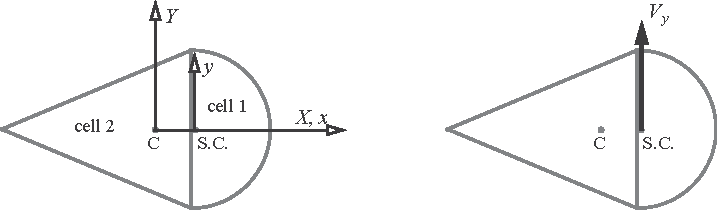
\includegraphics{Figure_4-39.pdf}}
\caption{Closed cross section consisting of two cells subject to transverse bending\label{fig4.39}}
\end{figure}
}


\begin{table}[H]
\vspace*{-12pt}
\processtable{Parametric equations of the contour\label{tab4.5}}{%
\tabcolsep=8pt\begin{tabular}{@{}llll@{}}
\toprule
\colhead{{$i$th} branch} & \colhead{$X_{i}(s) =$} & \colhead{$Y_{i}(s) =$} &
\colhead{Range}\\
\midrule
$i = 1$ & $a \sin \left(s_{1}/a\right)$  & $-a \cos \left(s_{1}/a\right)$ & $0 \leq s_{1} \leq a \pi$\\
$i = 2$ & $-b\left(s_{2}/c\right)$ & $a\left(1-s_{2}/c\right)$ & $0 \leq s_{2} \leq c$\\
$i = 3$ & $-b\left(1-s_{3}/c\right)$ & $-a\left(s_{3}/c\right)$ & $0 \leq s_{3} \leq c$\\
$i = 1-2$ & $0$ & $a-s_{\textrm{1-2}}$ & $0 \leq s_{\textrm{1-2}} \leq 2 a$\\
\botrule
\end{tabular}}{}
\vspace*{-1.6\baselineskip}
\end{table}

The cross-sectional area \textit{A}, first area moment ${Q}_Y$, and location of the centroid ${X}_c$ are computed as follows:
\begin{align}
A &=\int_{0}^{a \pi} t d s_{1}+\int_{0}^{c} t d s_{2}+\int_{0}^{c} t d s_{3}+\int_{0}^{2a}(t/2) d s_{\textrm{1-2}}=(a \pi+2 c+a) t=1.86832\,\mathrm{in}.^{2}\label{ex4.12a}\\
Q_{Y} &=\int_{0}^{a \pi} X_{1} t d s_{1}+\int_{0}^{c} X_{2} t d s_{2}+\int_{0}^{c} X_{3} t d s_{3}+\int_{0}^{2a} X_{12}(t/ 2) d s_{1-s}=(2 a^{2}-b c) t=-4.24\,\textrm{in}.^{3}\label{ex4.12b}\\
X_{c} &=Q_{Y}/A=-2.26942\,\textrm{in}.\label{ex4.12c}
\end{align}
Symmetry about \textit{X}-axis results in $Q_{X}=0$, so that $Y_{c}=0$. The Cartesian coordinates of the branches with respect to the centroid are $x_{i}\left(s_{i}\right)=X_{i}\left(s_{i}\right)-X_{c}$, and $y_{i}\left(s_{i}\right)=Y_{i}\left(s_{i}\right)$, $i=1,2,3,1$-$2$. The second area moment about the $x$-axis is
\begin{align}\label{ex4.12d}
I_{x x}=\int_{0}^{a \pi} y_{1}^{2} t d s_{1}+\int_{0}^{c} y_{2}^{2} t d s_{2}+\int_{0}^{c} y_{3}^{2} t d s_{3}+\int_{0}^{2a} y_{12}^{2}(t/2) d s_{\textrm{1-2}}=\frac{\pi a^{3} t}{2}+\frac{2 a^{2} c t}{3}+\frac{a^{3} t}{3}=18.1873\,\textrm{in}.^{4}.
\end{align}

The shear flow is given by eq.~(\ref{eq4.15}) on page \pageref{eq4.15}, and it is repeated as eq. (\textbf{\ref{ex4.12e}}) below.
\begin{align}\label{ex4.12e}
q(s, z)=q_{0}(z)-\frac{k}{I_{y y}} V_{x} \bar{Q}_{y}(s)-\frac{k}{I_{x x}} V_{y} \bar{Q}_{x}(s).
\end{align}
In this example the product area moment $I_{x y}=0$. From eq.~(\ref{eq4.4}) cross-sectional coefficients $n_{x}=n_{y}=0$ and $k=1$. The distribution function defined in eq.~(\ref{eq4.9}) simplifies to $\bar{Q}_{x}(s)=Q_{x}(s)$ since $\bar{y}(s)=y(s)$. Hence, the shear flow equation in the \textit{i-th} branch reduces to the form
\begin{align}\label{ex4.12f}
q_{i}\left(s_{i}\right)=q_{0 i}-\left(V_{y}/I_{x x}\right) Q_{x i}\left(s_{i}\right).
\end{align}
At the contour origin of the $i$-\textit{th} branch where $s_{i}=0$ the shear flow in eq. (\textbf{\ref{ex4.12f}}) is denoted by $q_{0 i}$, and the distribution function is given by
\begin{align}\label{ex4.12g}
Q_{x i}\left(s_{i}\right)=\int_{0}^{s_{i}} y_{i}\left(s_{i}\right) t_{i} d s_{i} \quad i=1,2,3,\textrm{1-2}.
\end{align}
\begin{wrapfigure}[10]{L}{122pt}
\vspace{-19pt}
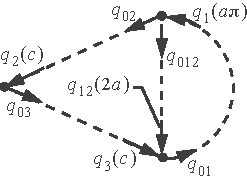
\includegraphics{Figure_4-40.pdf}
\caption{Junction shear flows.\label{fig4.40}}
\end{wrapfigure}

\removelastskip

\noindent Axial equilibrium per unit $z$-length at the three junctions connecting the branches leads to
\begin{align}\label{ex4.12h}
q_{1}(a \pi)=q_{02}+q_{012} \quad q_{2}(c)=q_{03} \quad q_{\textrm{1-2}}(2 a)+q_{3}(c)=q_{01}.
\end{align}
The shear flows acting at the three junctions are shown in figure~\ref{fig4.40}. We use the first two expressions in eq. (\textbf{\ref{ex4.12h}}) to eliminate $q_{012}$ and $q_{03}$. After computing the first area moment functions, the shear flows are as follows:
\begin{align}
q_{1}\left(s_{1}\right)&=q_{01}+\left(V_{y}/I_{x x}\right) a^{2} t \sin \left(s_{1}/a\right)\label{ex4.12i}\\
q_{2}\left(s_{2}\right)&=q_{02}-\left(V_{y}/I_{x x}\right)\left[a t s_{2}-\frac{a t s_{2}^{2}}{2 c}\right]\label{ex4.12j} \\
q_{3}\left(s_{3}\right)&=q_{02}-\left(V_{y}/I_{x x}\right)\left[\frac{a c t}{2}-\frac{a t s_{3}^{2}}{2 c}\right]\label{ex4.12k}\\
q_{\textrm{1-2}}\left(s_{\textrm{1-2}}\right)&=q_{01}-q_{02}-\left(V_{y}/I_{x x}\right)\left[\frac{a t s_{\textrm{1-2}}}{2}-\frac{t s_{\textrm{1-2}}^{2}}{4}\right].\label{ex4.12l}
\end{align}
Note: If eqs. (\textbf{\ref{ex4.12k}}) and (\textbf{\ref{ex4.12l}}) are substituted into the third junction condition of eq. (\textbf{\ref{ex4.12h}}), then we obtain the identity $q_{01}=q_{01}$. Hence, the shear flows from the axial equilibrium conditions contain two unknowns $q_{01}$ and $q_{02}$.

The resultant force acting on the section from the shear flows is given by the general relation
\begin{align}\label{ex4.12m}
F_{X} \hat{i}+F_{Y} \hat{j}=\int_{c} q \hat{t} d s=\left[\int_{c} q \frac{d x}{d s} d s\right] \hat{i}
+\left[\int_{c} q \frac{d y}{d s} d s\right]\hat{j}.
\end{align}
\vspace*{5pt}
\clearpage

\noindent Evaluation of the resultant forces gives
\begin{align}
F_{X} &=\int_{0}^{a \pi} q_{1}\left(\frac{d x_{1}}{d s_{1}}\right) d s_{1}+\int_{0}^{c} q_{2}\left(\frac{d x_{2}}{d s_{2}}\right) d s_{2}+\int_{0}^{c} q_{3}\left(\frac{d x_{3}}{d s_{3}}\right) d s_{3}+\int_{0}^{2a} q_{\textrm{1-2}}\left(\frac{d x_{12}}{d s_{12}}\right) d s_{\textrm{1-2}}=0, \text{and}\label{ex4.12n}
\\
F_{Y} &=\int_{0}^{a \pi} q_{1}\left(\frac{d y_{1}}{d s_{1}}\right) d s_{1}+\int_{0}^{c} q_{2}\left(\frac{d y_{2}}{d s_{2}}\right) d s_{2}+\int_{0}^{c} q_{3}\left(\frac{d y_{3}}{d s_{3}}\right) d s_{3}+\int_{0}^{2a} q_{\textrm{1-2}}\left(\frac{d y_{12}}{d s_{12}}\right) d s_{\textrm{1-2}}=V_{y}.\label{ex4.12o}
\end{align}
The shear flow is statically equivalent to the shear force, as expected. No new information to determine $q_{01}$ and $q_{02}$ is obtained. The shear force acting at the shear center implies the twist per unit axial length of the cross section vanishes. This condition leads to two equations governing the shear flows in each cell. For a uniform shear modulus the twist per unit length is
\begin{align}\label{ex4.12p}
\frac{d \phi_{z}}{d z}=\frac{1}{2 A_{c} G} \oint\! \frac{q}{t} d s.
\end{align}
Evaluate the twist per unit length for each cell and equate them to zero:
\begin{gather}\label{ex4.12q}
\left(\left.\frac{d \phi_{z}}{d z}\right|_{\textrm{cell } 1}=0\right) \rightarrow \frac{1}{t} \int_{0}^{a \pi} q_{1} d s_{1}+\frac{2}{t} \int_{0}^{2a} q_{\textrm{1-2}} d s_{\textrm{1-2}}=0
\\
\left(\left.\frac{{d} \phi_{z}}{{d} z}\right|_{\textrm{cell } 2}=0\right) \rightarrow \frac{1}{t} \int_{0}^{c} q_{2} d s_{2}+\frac{1}{t} \int_{0}^{c} q_{3} d s_{3}+\frac{2}{t} \int_{2 a}^{0} q_{\textrm{1-2}} d s_{\textrm{1-2}}=0\label{ex4.12r}
\end{gather}
Evaluation of eqs. (\textbf{\ref{ex4.12q}}) and (\textbf{\ref{ex4.12r}}), respectively, results in
\begin{gather}
\frac{a}{t}(4+\pi) q_{01}-\frac{4 a}{t} q_{02}+\frac{4 a^{3}}{3 I_{x x}} V_{y}=0, \text{and}\label{ex4.12s}\\
-\frac{4 a}{t} q_{01}+\frac{2(2 a+c)}{t} q_{02}-\frac{2 a b^{2}}{3 I_{x x}} V_{y}=0.\label{ex4.12t}
\end{gather}
Solve eqs. (\textbf{\ref{ex4.12s}}) and (\textbf{\ref{ex4.12t}}) for the shear flows $q_{01}$ and $q_{02}$ to get
\begin{gather}\label{ex4.12u}
q_{01}=\frac{-4 a t(3 a^{2}+a c-c^{2})}{(4 c+2 a \pi+c \pi)} \frac{V_{y}}{3 I_{x x}}=(3.42199 \times 10^{-3}\,\textrm{in}.^{-1}) V_{y}, \text{ and}\\[7pt]
q_{02}=\frac{-t(12 a^{3}-4 a c^{2}+a^{3} \pi-a c^{2} \pi)}{(4 c+2 a \pi+c \pi)} \frac{V_{y}}{3 I_{x x}}=(24.4374 \times 10^{-3}\,\textrm{in}.^{-1}) V_{y}.\label{ex4.12v}
\end{gather}
The final result for the shear flows are listed in eqs. (\textbf{\ref{ex4.12w}}) to (\textbf{\ref{ex4.12z}}) below.
\begin{align}
q_{1} &=\big[3.42199 \times 10^{-3}\,\textrm{in}.^{-1}+(54.9834 \times 10^{-3}\,\textrm{in}.^{-1}) \sin (s_{1}/5)\big] V_{y}\nonumber\\
&\quad 0 \leq s_{1} \leq 5 \pi\label{ex4.12w}\\[6pt]
q_{2}&=\big[24.4374 \times 10^{-3}\,\textrm{in}.^{-1}-(10.9967 \times 10^{3}\,\textrm{in}.^{-2}) s_{2}+(0.422949 \times 10^{-3}\,\textrm{in}.^{-3}) s_{2}^{2}\big] V_{y}\nonumber\\
& \quad 0 \leq s_{2} \leq 13\,\textrm{in}. \label{ex4.12x}\\[6pt]
q_{3}&=\big[-47.041 \times 10^{-3}\,\textrm{in}.^{-1}+(0.433949 \times 10^{-3}\,\textrm{in}.^{-3}) s_{3}^{2}\big] V_{y}\nonumber\\
& \quad 0 \leq s_{3} \leq 13\,\textrm{in}.\label{ex4.12y}\\[6pt]
q_{\textrm{1-2}}&=\big[-21.0154 \times 10^{-3}\,\textrm{in}.^{-1}-(5.49834 \times 10^{-3}\,\textrm{in}.^{-2}) s_{\textrm{1-2}}+(5.49834 \times 10^{-3}\,\textrm{in}.^{-3}) s_{\textrm{1-2}}^{2}\big] V_{y}\nonumber\\
& \quad 0 \leq s_{\textrm{1-2}} \leq 10\,\textrm{in}.\label{ex4.12z}
\end{align}

With the shear flows known we compute the torque about the centroid due to the shear flows by
\setcounter{equation}{0}\def\theequation{a\alph{equation}}
\begin{align}\label{ex4.12aa}
M_{z c}=\int_{0}^{a \pi} r_{n c 1} q_{1} d s_{1}+\int_{0}^{c} r_{n c 2} q_{2} d s_{2}+\int_{0}^{c} r_{n c 3} q_{3} d s_{3}+\int_{0}^{2a} r_{n c 12} q_{\textrm{1-2}} d s_{\textrm{1-2}},\tag{aa}
\end{align}
where $r_{n c i}\left(s_{i}\right)$ is the normal coordinate to the contour with respect to the centroid in the $i$-th branch. From eq.~(\ref{eq4.10}) the normal coordinates are determined from
\begin{align}\label{ex4.12ab}
r_{n c i}=x_{i}\left(s_{i}\right) \frac{d y_{i}}{d s_{i}}-y_{i}\left(s_{i}\right) \frac{d x_{i}}{d s_{i}}.\tag{ab}
\end{align}
The results for the normal coordinates are
\begin{align}\label{ex4.12ac}
r_{n c 1}=a-X_{c} \sin \left(s_{1}/a\right) \quad r_{n c 2}=a\left(b+X_{c}\right)/c \quad r_{n c 3}=a\left(b+X_{c}\right)/c \quad r_{n c 1\mbox{-}2}=X_{c}.\tag{ac}
\end{align}
Substitute eqs. (\textbf{\ref{ex4.12w}}) to (\textbf{\ref{ex4.12z}}) for the shear flows into eq. (\textbf{\ref{ex4.12y}}), followed by substitution of eq. (\textbf{\ref{ex4.12ac}}) for the normal coordinates. Numerical evaluation of the integrals after the substitutions leads to the expression for the torque in the form
\begin{align}\label{ex4.12ad}
M_{z c}=(2.50157\,\textrm{in}.) V_{y}.\tag{ad}
\end{align}
The resultant force and torque at the centroid are shown in figure~\ref{fig4.41}(a). We also added and subtracted the shear force at the shear center in figure~\ref{fig4.41}(a), which does not change the static state. The upward shear force at the centroid and the downward shear force at the shear center form a clockwise couple whose moment is $x_{s c} V_{y}$. In figure~\ref{fig4.41}(b) we resolved the torque $M_{z}=(2.50157\,\textrm{in}.) V_{y}-x_{s c} V_{y}$ and shear force at the shear center. Since the torque at the shear center is equal to zero in this case, we can solve for the shear center location relative to the centroid to get
\begin{align}\label{ex4.12ae}
x_{s c}=2.50157\,\textrm{in}.\tag{ae}
\end{align}

{\def\thefigure{4.41}
\processfigure[H]{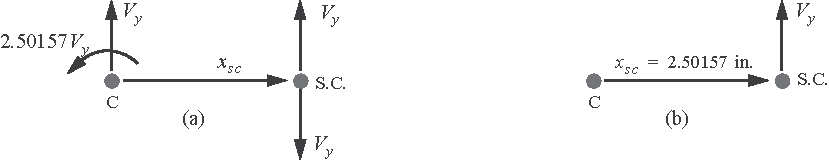
\includegraphics{Figure_4-41.pdf}
}{\caption{(a) Resultant of the shear flows at the centroid. (b) Resultant of the shear flows at the shear center.\label{fig4.41}}}}

We perform one last check on the solution by computing the torque at the shear due to the shear flows from the equation
\begin{align}\label{ex4.12af}
M_{z}=\int_{0}^{a \pi} r_{n 1} q_{1} d s_{1}+\int_{0}^{c} r_{n 2} q_{2} d s_{2}+\int_{0}^{c} r_{n 3} q_{3} d s_{3}+\int_{0}^{2a} r_{n 12} q_{\textrm{1-2}} d s_{\textrm{1-2}},\tag{af}
\end{align}
\vspace*{5pt}
\clearpage

\noindent where the coordinates normal to contour with respect to the shear center are denoted by $r_{n i}\left(s_{i}\right)$. From eq.~(\ref{eq3.10}) on page \pageref{eq3.10} the normal coordinates are related by
\begin{align}\label{ex4.12ag}
r_{n i}=r_{n c i}-x_{s c} \frac{d y_{i}}{d s_{i}}+y_{s c} \frac{d x_{i}}{d s_{i}}.\tag{ag}
\end{align}
In this example $y_{s c}=0$, and the results for the coordinates $r_{n i}\left(s_{i}\right)$ are given in eqs. (\textbf{\ref{ex4.12ah}}) and (\textbf{\ref{ex4.12ai}}) below.
\begin{gather}
r_{n 1}=r_{n c 1}-x_{s c}\left(\frac{\partial y_{1}}{\partial s_{1}}\right)=5-0.232149 \sin \left(s_{1}/5\right) \quad r_{n 2}=r_{n c 2}-x_{s c}\left(\frac{\partial y_{2}}{\partial s_{2}}\right)=4.70467\,\textrm{in}.
\label{ex4.12ah}\tag{ah}\\
r_{n 3}=r_{n c 3}-x_{s c}\left(\frac{\partial y_{3}}{\partial s_{3}}\right)=4.70467\,\textrm{in. } \quad r_{n 1\mbox{-}2}=r_{n c 1\mbox{-}2}-x_{s c}\left(\frac{\partial y_{\textrm{1-2}}}{\partial s_{\textrm{1-2}}}\right)=0.232149\,\textrm{in}.\label{ex4.12ai}\tag{ai}
\end{gather}
Substitute the shear flows from eqs. (\textbf{\ref{ex4.12w}}) to (\textbf{\ref{ex4.12z}}) into eq. (\textbf{\ref{ex4.12af}}), followed by the substitution of the coordinates normal to the contour in eqs. (\textbf{\ref{ex4.12ah}}) and (\textbf{\ref{ex4.12ai}}). After these substitutions we perform the integrations indicated in eq. (\textbf{\ref{ex4.12af}}) to find the result for torque at the shear center as
\begin{align}\label{ex4.12aj}\tag{aj}
M_{z}=\left(-1.421 \times 10^{-14}\right) \frac{V_{y}}{I_{x x}} \approx 0.
\end{align}
Hence, the numerical result for the torque at the shear center with respect to finite precision arithmetic is equal to zero\footnote{All computations performed numerically in a computer (MatLab, Mathematica, etc.) are performed with finite precision. That is, a decimal representation of a number that has been rounded or truncated. Computations performed numerically with decimal, or decimal floating point, representation are referred to as finite precision arithmetic.}.
\end{example}

\begin{wrapfigure}[10]{r}{116pt}
%\vspace{-19pt}
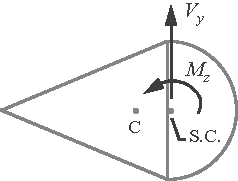
\includegraphics{Figure_4-42.pdf}
\caption{shear and torsion of the two-cell section.\label{fig4.42}}
\end{wrapfigure}

\begin{example*}[Superposition of example \ref{ex4.10} and example \ref{ex4.12}]\label{ex14.13}\setcounter{equation}{0}\def\theequation{\alph{equation}}%
Now consider that the cross section of example \ref{ex4.10} and example \ref{ex4.12} is subject to a torque $M_{z}$ and a shear force $V_{y}$ at the shear center as shown in figure~\ref{fig4.42}. We simply add the results for the shear flows due to the torque from example \ref{ex4.10} to the shear flows due to the transverse shear force $V_{y}$ from example \ref{ex4.12}.

The results are
\begin{align*}
q_{1}(s_{1})&=(0.0040053\,\textrm{in}.^{-2}) M_{z}+\left[0.00342199\,\textrm{in}.^{-1}+(0.0549834\,\textrm{in}.^{-1})\right.\\[4pt]
&\quad \left.\sin (s_{1}/5)\right] V_{y}, 0 \leq s_{1} \leq(5 \pi)\,\textrm{in}.,\\[4pt]
q_{2}(s_{2})&=(0.00300903\,\textrm{in}.^{-2}) M_{z}+\left[0.0244374\,\textrm{in}.^{-1}-(0.0109967\,\textrm{in}.^{-2}) s_{2}\right.\\[4pt]
&\quad +\left.(0.000422949\,\textrm{in}.^{-3}) s_{2}^{2}\right] V_{y},\quad 0 \leq s_{2} \leq 13\,\textrm{in}.\\[4pt]
q_{3}(s_{3})&=(0.00300903\,\textrm{in}.^{-2})\; M_{z}+\left[-0.047041\,\textrm{in}.^{-1}+(0.000422949\,\textrm{in}.^{-3}) s_{3}^{2}\right] V_{y} \quad 0 \leq s_{3} \leq 13\,\textrm{in}., \text{ and}\\[4pt]
q_{\textrm{1-2}}(s_{\textrm{1-2}})&=(0.000915085\,\textrm{in}.^{-2}) M_{z}+\left[-0.0210154\,\textrm{in}.^{-1}-(0.00549834\,\textrm{in}.^{-2}) s_{\textrm{1-2}}\right.\\[4pt]
&\quad +\left.(0.00549834\,\textrm{in}.^{-3}) s_{\textrm{1-2}}^{2}\right] V_{y}\quad 0 \leq s_{\textrm{1-2}} \leq 10\,\textrm{in}.
\end{align*}
\end{example*}

\begin{thebibliography}{}\label{sec4.5}
\bibitem{} Dowling, N. E. \textit{\textbf{Mechanical Behavior of Materials}}: Engineering Methods for Deformation, Fracture, and Fatigue. Englewood Cliffs, NJ: Prentice Hall, 1993, Chapter 7.\label{Dowling}

\bibitem{} Muckle, W. \textit{\textbf{Strength of Ships' Structures}}. London: Edward Arnold, Inc., 1967, pp. 5--12, 27--69.

\bibitem{} Zubaly, R.M. \textit{\textbf{Applied Naval Architecture}}. The Society of Naval Architects and Marine Engineers and Cornell Maritime Press, Inc., 1996, pp. 195--237.
\end{thebibliography}

\vspace*{-15pt}
\section{Practice exercises}\label{sec4.6}

\begin{exercise}
\begin{enumerate}[\textbf{2.}]
\item[\textbf{1.}] A 7\,m long AH-1W Supercobra helicopter blade is rotating at 300\,rpm and has a mass of 300\,kg. Centrifugal forces due to the rotation of the blade lead to tension in the blade. Plot the distributed axial force intensity and the internal axial force distribution on the blade. Calculate the stress at the root for a blade cross-sectional area of $0.02\,\textrm{m}^2$. (Assume that the mass is evenly distributed and the center of mass of the cross section coincides with the tension axis.)

\item[\textbf{2.}] The cantilever wing is subject to a distributed air load $f_{y}(z)=\frac{2 L}{\pi z_{\textit{max}}} \sqrt{1-(\bar{z})^{2}}$, where the total lift (2 wings) $L=20{,}000\,\textrm{lb.}$ at cruise, wing length $z_{\textit{max}}=32.5\,\textrm{ft.}$, and ${\bar{z}}=z/z_{\textit{max}}$. Also, the wing supports an engine weighing 1000~lb. See figure~\ref{fig4.43}. Plot the loading diagram, shear force diagram $V_{y}(z)$, and bending moment diagram $M_{x}(z)$ as functions of \textit{z} for $0\leq z \leq 32.5$ ft. Partial answer: $V_{y}(0) = 9{,}000$~lb. and $M_{x}(0)= -131{,}934$\,lb.-ft.\vspace*{-6pt}

{\def\thefigure{4.43}
\processfigure[H]{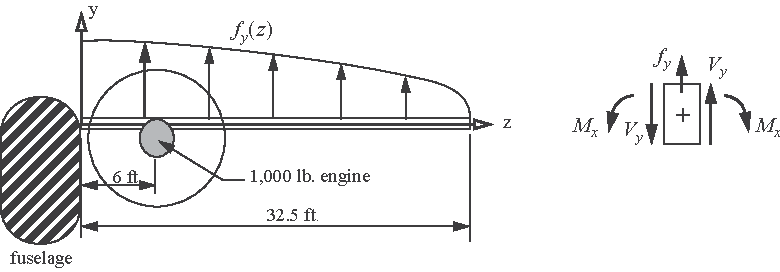
\includegraphics{Figure_4-43.pdf}
}{\caption{Exercise 3.\label{fig4.43}}}}

\vspace*{-13pt}

\item[\textbf{3.}] The barge shown figure~\ref{fig4.44} is 20\,m long and has a uniform cross section along its length that is the same cross section shown in figure~\ref{fig4.11} on page \pageref{fig4.11}. It is subject to a uniformly distributed downward load with{\parfillskip=0pt\par}\vspace*{-6pt}

{\def\thefigure{4.44}
\begin{figure}[H]
\centering{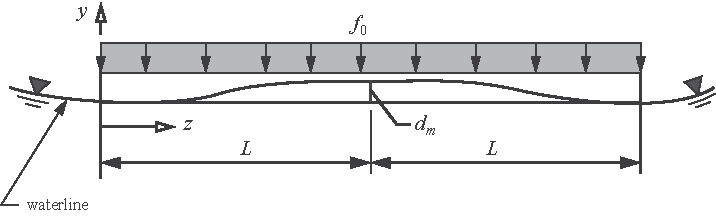
\includegraphics{Figure_4-44.pdf}}
\caption{Barge in a hogging condition.\label{fig4.44}}\vspace*{-10pt}
\end{figure}
}

\pagebreak

{\def\thefigure{4.45}
\begin{figure}[!b]\vspace*{-17pt}
\centering{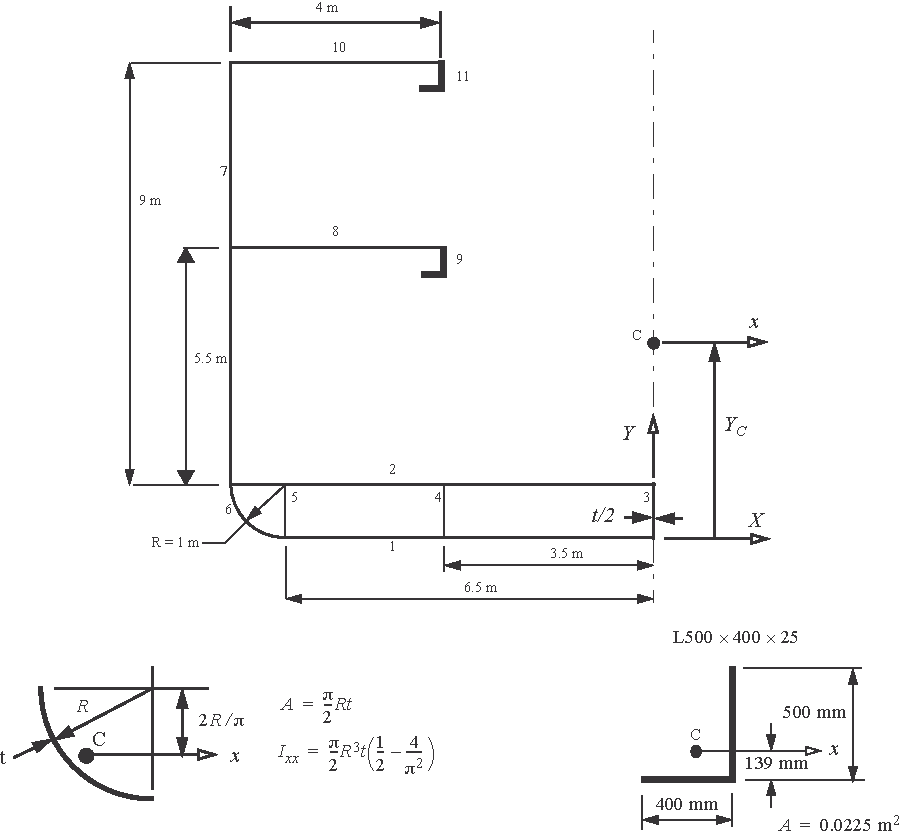
\includegraphics{Figure_4-45.pdf}}
\caption{Exercise 4. Ship half section.\label{fig4.45}}\vspace*{-6pt}
\end{figure}}


\noindent intensity $f_{0}=100\,\textrm{kN}/\textrm{m}$, and a buoyancy distribution in the hogging condition. The buoyancy distribution is given by $f_{b}=\gamma b d_{m}\left[1-\cos \left(\pi \frac{z}{L}\right)\right]$,where $\gamma = 9.8\,\textrm{kN/m}^3$ is the specific weight of water, $b=10$\,m, $d_{m}$ is the depth of the immersed cross section amidships, and $L=10$~m. Refer to figure~\ref{fig4.44}
\begin{enumerate}[b)]
  \item[a)] Determine $d_{m}$.
  \item[b)] Determine the distributed loading intensity function $f_{y}(z)$ for $0 \leq z \leq 20~\mathrm{m}$
  \item[c)] Determine the shear force $V_{y}(z)$ and bending moment $M_{x}(z)$ for $0 \leq z \leq 20~\mathrm{m}$.
  \item[d)] Draw the distributed loading intensity, shear force, and bending moment diagrams in the manner shown\break\hspace*{21pt} in figure~\ref{fig4.10} on page~\pageref{fig4.10}. Label significant points.
  \item[e)] Determine the maximum value of the normal stress $\sigma_{z z}$.
\end{enumerate}

\item[\textbf{4.}]  Half of the cross section of a ship is shown in figure~\ref{fig4.45}. Only the material that is effective in the longitudinal bending is illustrated in the figure. Determine the area \textit{A}, location of the centroid $Y_{C}$, and the second area moment{\parfillskip=0pt\par}

\clearpage

\noindent about the $x$-axis($I_{x x}$) for the \textit{full} section. Use the tabular format for the computations similar to table \ref{tab4.2} on page \pageref{tab4.2}. All plating has a thickness $t = 14$\,mm unless other wise noted. The descriptions of the numbered structural elements shown in the figure are listed in table \ref{tab4.6}.

\begin{table}[h]%Table 4.6
\processtable{Description of structural member in figure~\ref{fig4.45}. \label{tab4.6}}{%
\tabcolsep=42pt
\begin{tabular}{@{}ll@{}}
\toprule
\colhead{\textbf{Item \#}} & \colhead{\textbf{Description}}\\
\midrule
1 & Outer bottom\\
2 & Inner bottom\\
3 & Center girder\\
4 \& 5 & Side girders\\
6 & Bilge (curved portion)\\
7 & Side plating\\
8 & Second deck plating\\
9 \& 11 & Hatch side girders L~$500 \times 400 \times 25$\\
10 & Strength deck plating\\
\botrule
\end{tabular}}{\vspace*{-16pt}}
\end{table}


\item[\textbf{5.}]  The thickness of each branch in the thin-walled cross section shown in figure~\ref{fig4.46} is 3\,mm and $I_{x x}=10^{5}\,\textrm{mm}^{4}$. The shear force $V_{y}=5\,\textrm{kN}$.





\begin{enumerate}[b)]
  \item[a)] Determine the shear flow distribution and sketch it on the cross section. Indicate on the sketch the positive sense along the branch.
  \item[b)] Estimate the shear stress due to the transverse shear force at point \textit{A}.
  \item[c)] Estimate the maximum shear stress due to transverse shear.
\end{enumerate}


\item[\textbf{6.}]  The cross section shown in figure~\ref{fig4.46} is subject to a vertical shear force $V_{y}$, positive upward, and a counterclockwise torque $M_{z}$ acting at the shear center. Take dimensions $b=40~\mathrm{mm}$ and $t=0.635~\mathrm{mm}$ Determine torsion constant \textit{J} and the magnitude of the maximum shear stress $\left(\sigma_{z s}\right)_{max}$.

{\def\thefigure{4.46}
\processfigure[H]{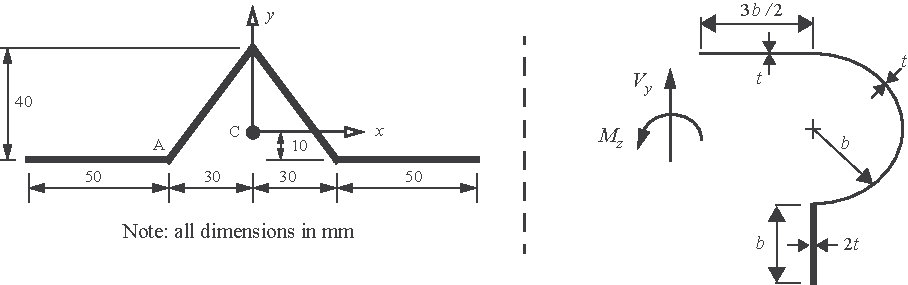
\includegraphics{Figure_4-46.pdf}
}{\caption{Exercise 5.\hspace*{15pc} Exercise 6.\hspace*{-2pc}\label{fig4.46}}}}

\clearpage

\item[\textbf{7.}]  Determine the shear flow in two-cell cross section shown in figure~\ref{fig4.47}. The \textit{X}-axis is a horizontal axis of symmetry,

{\def\thefigure{4.47}
\processfigure[H]{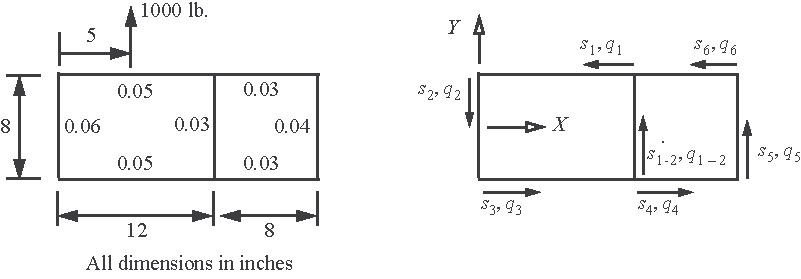
\includegraphics{Figure_4-47.pdf}
}{\caption{Two-cell box cross section.\label{fig4.47}}}}
\end{enumerate}
\end{exercise}

\clearemptydoublepage

\end{document} 